%Version 3.1 December 2024
% See section 11 of the User Manual for version history
%
%%%%%%%%%%%%%%%%%%%%%%%%%%%%%%%%%%%%%%%%%%%%%%%%%%%%%%%%%%%%%%%%%%%%%%
%%                                                                 %%
%% Please do not use \input{...} to include other tex files.       %%
%% Submit your LaTeX manuscript as one .tex document.              %%
%%                                                                 %%
%% All additional figures and files should be attached             %%
%% separately and not embedded in the \TeX\ document itself.       %%
%%                                                                 %%
%%%%%%%%%%%%%%%%%%%%%%%%%%%%%%%%%%%%%%%%%%%%%%%%%%%%%%%%%%%%%%%%%%%%%

%%\documentclass[referee,sn-basic]{sn-jnl}% referee option is meant for double line spacing

%%=======================================================%%
%% to print line numbers in the margin use lineno option %%
%%=======================================================%%

%%\documentclass[lineno,pdflatex,sn-basic]{sn-jnl}% Basic Springer Nature Reference Style/Chemistry Reference Style

%%=========================================================================================%%
%% the documentclass is set to pdflatex as default. You can delete it if not appropriate.  %%
%%=========================================================================================%%

%%\documentclass[sn-basic]{sn-jnl}% Basic Springer Nature Reference Style/Chemistry Reference Style

%%Note: the following reference styles support Namedate and Numbered referencing. By default the style follows the most common style. To switch between the options you can add or remove “Numbered” in the optional parenthesis. 
%%The option is available for: sn-basic.bst, sn-chicago.bst%  
 
%%\documentclass[pdflatex,sn-nature]{sn-jnl}% Style for submissions to Nature Portfolio journals
%%\documentclass[pdflatex,sn-basic]{sn-jnl}% Basic Springer Nature Reference Style/Chemistry Reference Style
\documentclass[pdflatex,sn-mathphys-num]{sn-jnl}% Math and Physical Sciences Numbered Reference Style
%%\documentclass[pdflatex,sn-mathphys-ay]{sn-jnl}% Math and Physical Sciences Author Year Reference Style
%%\documentclass[pdflatex,sn-aps]{sn-jnl}% American Physical Society (APS) Reference Style
%%\documentclass[pdflatex,sn-vancouver-num]{sn-jnl}% Vancouver Numbered Reference Style
%%\documentclass[pdflatex,sn-vancouver-ay]{sn-jnl}% Vancouver Author Year Reference Style
%%\documentclass[pdflatex,sn-apa]{sn-jnl}% APA Reference Style
%%\documentclass[pdflatex,sn-chicago]{sn-jnl}% Chicago-based Humanities Reference Style

%%%% Standard Packages
%%<additional latex packages if required can be included here>

\usepackage{graphicx}%
\usepackage{multirow}%
\usepackage{amsmath,amssymb,amsfonts}%
\usepackage{amsthm}%
\usepackage{mathrsfs}%
\usepackage[title]{appendix}%
\usepackage{xcolor}%
\usepackage{textcomp}%
\usepackage{manyfoot}%
\usepackage{booktabs}%
\usepackage{subcaption}
\usepackage{algorithm}%
\usepackage{algorithmicx}%
\usepackage{algpseudocode}%
\usepackage{listings}%
%%%%

%%%%%=============================================================================%%%%
%%%%  Remarks: This template is provided to aid authors with the preparation
%%%%  of original research articles intended for submission to journals published 
%%%%  by Springer Nature. The guidance has been prepared in partnership with 
%%%%  production teams to conform to Springer Nature technical requirements. 
%%%%  Editorial and presentation requirements differ among journal portfolios and 
%%%%  research disciplines. You may find sections in this template are irrelevant 
%%%%  to your work and are empowered to omit any such section if allowed by the 
%%%%  journal you intend to submit to. The submission guidelines and policies 
%%%%  of the journal take precedence. A detailed User Manual is available in the 
%%%%  template package for technical guidance.
%%%%%=============================================================================%%%%

%% as per the requirement new theorem styles can be included as shown below
\theoremstyle{thmstyleone}%
\newtheorem{theorem}{Theorem}%  meant for continuous numbers
%%\newtheorem{theorem}{Theorem}[section]% meant for sectionwise numbers
%% optional argument [theorem] produces theorem numbering sequence instead of independent numbers for Proposition
\newtheorem{proposition}[theorem]{Proposition}% 
%%\newtheorem{proposition}{Proposition}% to get separate numbers for theorem and proposition etc.

\theoremstyle{thmstyletwo}%
\newtheorem{example}{Example}%
\newtheorem{remark}{Remark}%

\theoremstyle{thmstylethree}%
\newtheorem{definition}{Definition}%

\raggedbottom
%%\unnumbered% uncomment this for unnumbered level heads

\begin{document}

\title[Article Title]{Proposal of a novel biomarker for neonatal seizure detection}

%%=============================================================%%
%% GivenName	-> \fnm{Joergen W.}
%% Particle	-> \spfx{van der} -> surname prefix
%% FamilyName	-> \sur{Ploeg}
%% Suffix	-> \sfx{IV}
%% \author*[1,2]{\fnm{Joergen W.} \spfx{van der} \sur{Ploeg} 
%%  \sfx{IV}}\email{iauthor@gmail.com}
%%=============================================================%%

\author*[1,2]{\fnm{First} \sur{Author}}\email{iauthor@gmail.com}

\author[2,3]{\fnm{Second} \sur{Author}}\email{iiauthor@gmail.com}
\equalcont{These authors contributed equally to this work.}

\author[1,2]{\fnm{Third} \sur{Author}}\email{iiiauthor@gmail.com}
\equalcont{These authors contributed equally to this work.}

\affil*[1]{\orgdiv{Department}, \orgname{Organization}, \orgaddress{\street{Street}, \city{City}, \postcode{100190}, \state{State}, \country{Country}}}

\affil[2]{\orgdiv{Department}, \orgname{Organization}, \orgaddress{\street{Street}, \city{City}, \postcode{10587}, \state{State}, \country{Country}}}

\affil[3]{\orgdiv{Department}, \orgname{Organization}, \orgaddress{\street{Street}, \city{City}, \postcode{610101}, \state{State}, \country{Country}}}

%%==================================%%
%% Sample for unstructured abstract %%
%%==================================%%

\abstract{The abstract serves both as a general introduction to the topic and as a brief, non-technical summary of the main results and their implications. Authors are advised to check the author instructions for the journal they are submitting to for word limits and if structural elements like subheadings, citations, or equations are permitted.}

%%================================%%
%% Sample for structured abstract %%
%%================================%%

% \abstract{\textbf{Purpose:} The abstract serves both as a general introduction to the topic and as a brief, non-technical summary of the main results and their implications. The abstract must not include subheadings (unless expressly permitted in the journal's Instructions to Authors), equations or citations. As a guide the abstract should not exceed 200 words. Most journals do not set a hard limit however authors are advised to check the author instructions for the journal they are submitting to.
% 
% \textbf{Methods:} The abstract serves both as a general introduction to the topic and as a brief, non-technical summary of the main results and their implications. The abstract must not include subheadings (unless expressly permitted in the journal's Instructions to Authors), equations or citations. As a guide the abstract should not exceed 200 words. Most journals do not set a hard limit however authors are advised to check the author instructions for the journal they are submitting to.
% 
% \textbf{Results:} The abstract serves both as a general introduction to the topic and as a brief, non-technical summary of the main results and their implications. The abstract must not include subheadings (unless expressly permitted in the journal's Instructions to Authors), equations or citations. As a guide the abstract should not exceed 200 words. Most journals do not set a hard limit however authors are advised to check the author instructions for the journal they are submitting to.
% 
% \textbf{Conclusion:} The abstract serves both as a general introduction to the topic and as a brief, non-technical summary of the main results and their implications. The abstract must not include subheadings (unless expressly permitted in the journal's Instructions to Authors), equations or citations. As a guide the abstract should not exceed 200 words. Most journals do not set a hard limit however authors are advised to check the author instructions for the journal they are submitting to.}

\keywords{Neonatal seizures, Electroencephalography, Power spectral density, Empirical mode decomposition, Neural network, Biomarker}

%%\pacs[JEL Classification]{D8, H51}

%%\pacs[MSC Classification]{35A01, 65L10, 65L12, 65L20, 65L70}

\maketitle

\section{Introduction}\label{sec1}

Neonatal seizures represent the most frequent neurological emergency in the newborn period and are widely recognised as a hallmark of significant underlying brain dysfunction. With an estimated incidence of 1--5 per 1{,}000 live births in term neonates and substantially higher rates of 57--132 per 1{,}000 in preterm infants \cite{glass2016}, seizures occur more commonly during the neonatal period than at any other stage of life. The predominant aetiologies include hypoxic--ischaemic encephalopathy, intracranial haemorrhage, ischaemic stroke, central nervous system infections, and inborn errors of metabolism \cite{ronen2007}. Long-term follow-up studies have established that neonatal seizures are independently associated with adverse neurodevelopmental outcomes, predisposing affected infants to epilepsy, cerebral palsy, cognitive impairment, and behavioural disorders in later childhood \cite{glass2009}. Because the prognosis depends critically on rapid identification and treatment, there is a compelling clinical need for accurate and timely seizure detection.

Electroencephalography (EEG) is the accepted gold standard for diagnosing neonatal seizures \cite{shellhaas2011}. Scalp electrodes record the voltage differences produced by postsynaptic ionic currents, providing both the spatial and temporal resolution required to characterise seizure morphology, duration, and burden \cite{boylan2013}. Continuous EEG monitoring in the neonatal intensive care unit has revealed that the majority of electrographic seizures---by some estimates 60--80\%---are subclinical, exhibiting no outward clinical correlates and therefore escaping bedside recognition entirely \cite{murray2008}. Even when expert neurophysiologists review the recordings, inter-observer agreement remains only moderate; studies report significant discordance in seizure identification among clinicians with different levels of experience \cite{stevenson2015}. Manual interpretation is further constrained by its substantial time and labour requirements, rendering round-the-clock coverage impractical in many centres. These limitations collectively underscore the demand for automated, computer-aided seizure detection systems.

A diverse array of automated approaches has been investigated over the past two decades. Early methods relied on hand-crafted features drawn from the time, frequency, and time--frequency domains, which were subsequently classified by traditional machine learning algorithms such as support vector machines, random forests, and logistic regression \cite{temko2011}. Feature extraction strategies in this paradigm have included amplitude statistics, spectral band powers, wavelet coefficients, and autocorrelation measures \cite{greene2008}. Although these systems achieved reasonable sensitivity, they often suffered from high false-detection rates and limited generalisability across datasets and recording conditions.

More recently, deep learning architectures have been applied to neonatal seizure detection, offering end-to-end learning that can jointly optimise feature extraction and classification. Convolutional neural networks (CNNs) have demonstrated strong performance by automatically learning spatial and spectral representations from multichannel EEG \cite{ansari2019}. Hybrid frameworks combining CNNs with recurrent layers, such as Long Short-Term Memory (LSTM) networks, have also been proposed; for example, the integration of Discrete Wavelet Transform decomposition with a 1D-CNN--LSTM pipeline has been shown to outperform traditional classifiers on several benchmark datasets \cite{kashefiamiri2025}. In the few-shot learning setting, Empirical Mode Decomposition (EMD) has been used to decompose EEG signals into Intrinsic Mode Functions, enriching the time--frequency representation and enabling superior sensitivity even when training data are severely limited \cite{pan2024}. Despite these advances, the majority of deep learning methods operate as opaque end-to-end systems, offering limited interpretability regarding which physiological signal properties drive their decisions.

Parallel to the development of automated classifiers, a substantial body of work has investigated the spectral characteristics of the EEG as a source of physiologically meaningful biomarkers. Power spectral density (PSD) analysis quantifies how signal energy is distributed across frequency, and has been widely used to characterise brain-state changes during seizures. During neonatal seizures the PSD profile typically deviates from the characteristic $1/f^{-\alpha}$ power-law decay observed during normal rest and sleep, with seizure epochs exhibiting elevated power in specific frequency bands, particularly in the theta (3--12~Hz) range \cite{stevenson2017}. Band-specific power measures---for instance, delta power and total spectral power---have been employed to predict encephalopathy severity and to identify neonates at risk for seizures within the first hour of EEG recording \cite{lloyd2021}.


% \section{Results}\label{sec2}

% Sample body text. Sample body text. Sample body text. Sample body text. Sample body text. Sample body text. Sample body text. Sample body text.

% \section{This is an example for first level head---section head}\label{sec3}

% \subsection{This is an example for second level head---subsection head}\label{subsec2}

% \subsubsection{This is an example for third level head---subsubsection head}\label{subsubsec2}

% Sample body text. Sample body text. Sample body text. Sample body text. Sample body text. Sample body text. Sample body text. Sample body text. 

% \section{Equations}\label{sec4}

% Equations in \LaTeX\ can either be inline or on-a-line by itself (``display equations''). For
% inline equations use the \verb+$...$+ commands. E.g.: The equation
% $H\psi = E \psi$ is written via the command \verb+$H \psi = E \psi$+.

% For display equations (with auto generated equation numbers)
% one can use the equation or align environments:
% \begin{equation}
% \|\tilde{X}(k)\|^2 \leq\frac{\sum\limits_{i=1}^{p}\left\|\tilde{Y}_i(k)\right\|^2+\sum\limits_{j=1}^{q}\left\|\tilde{Z}_j(k)\right\|^2 }{p+q}.\label{eq1}
% \end{equation}
% where,
% \begin{align}
% D_\mu &=  \partial_\mu - ig \frac{\lambda^a}{2} A^a_\mu \nonumber \\
% F^a_{\mu\nu} &= \partial_\mu A^a_\nu - \partial_\nu A^a_\mu + g f^{abc} A^b_\mu A^a_\nu \label{eq2}
% \end{align}
% Notice the use of \verb+\nonumber+ in the align environment at the end
% of each line, except the last, so as not to produce equation numbers on
% lines where no equation numbers are required. The \verb+\label{}+ command
% should only be used at the last line of an align environment where
% \verb+\nonumber+ is not used.
% \begin{equation}
% Y_\infty = \left( \frac{m}{\textrm{GeV}} \right)^{-3}
%     \left[ 1 + \frac{3 \ln(m/\textrm{GeV})}{15}
%     + \frac{\ln(c_2/5)}{15} \right]
% \end{equation}
% The class file also supports the use of \verb+\mathbb{}+, \verb+\mathscr{}+ and
% \verb+\mathcal{}+ commands. As such \verb+\mathbb{R}+, \verb+\mathscr{R}+
% and \verb+\mathcal{R}+ produces $\mathbb{R}$, $\mathscr{R}$ and $\mathcal{R}$
% respectively (refer Subsubsection~\ref{subsubsec2}).

% \section{Tables}\label{sec5}

% Tables can be inserted via the normal table and tabular environment. To put
% footnotes inside tables you should use \verb+\footnotetext[]{...}+ tag.
% The footnote appears just below the table itself (refer Tables~\ref{tab1} and \ref{tab2}). 
% For the corresponding footnotemark use \verb+\footnotemark[...]+

% \begin{table}[h]
% \caption{Caption text}\label{tab1}%
% \begin{tabular}{@{}llll@{}}
% \toprule
% Column 1 & Column 2  & Column 3 & Column 4\\
% \midrule
% row 1    & data 1   & data 2  & data 3  \\
% row 2    & data 4   & data 5\footnotemark[1]  & data 6  \\
% row 3    & data 7   & data 8  & data 9\footnotemark[2]  \\
% \botrule
% \end{tabular}
% \footnotetext{Source: This is an example of table footnote. This is an example of table footnote.}
% \footnotetext[1]{Example for a first table footnote. This is an example of table footnote.}
% \footnotetext[2]{Example for a second table footnote. This is an example of table footnote.}
% \end{table}

% \noindent
% The input format for the above table is as follows:

% %%=============================================%%
% %% For presentation purpose, we have included  %%
% %% \bigskip command. Please ignore this.       %%
% %%=============================================%%
% \bigskip
% \begin{verbatim}
% \begin{table}[<placement-specifier>]
% \caption{<table-caption>}\label{<table-label>}%
% \begin{tabular}{@{}llll@{}}
% \toprule
% Column 1 & Column 2 & Column 3 & Column 4\\
% \midrule
% row 1 & data 1 & data 2	 & data 3 \\
% row 2 & data 4 & data 5\footnotemark[1] & data 6 \\
% row 3 & data 7 & data 8	 & data 9\footnotemark[2]\\
% \botrule
% \end{tabular}
% \footnotetext{Source: This is an example of table footnote. 
% This is an example of table footnote.}
% \footnotetext[1]{Example for a first table footnote.
% This is an example of table footnote.}
% \footnotetext[2]{Example for a second table footnote. 
% This is an example of table footnote.}
% \end{table}
% \end{verbatim}
% \bigskip
% %%=============================================%%
% %% For presentation purpose, we have included  %%
% %% \bigskip command. Please ignore this.       %%
% %%=============================================%%

% \begin{table}[h]
% \caption{Example of a lengthy table which is set to full textwidth}\label{tab2}
% \begin{tabular*}{\textwidth}{@{\extracolsep\fill}lcccccc}
% \toprule%
% & \multicolumn{3}{@{}c@{}}{Element 1\footnotemark[1]} & \multicolumn{3}{@{}c@{}}{Element 2\footnotemark[2]} \\\cmidrule{2-4}\cmidrule{5-7}%
% Project & Energy & $\sigma_{calc}$ & $\sigma_{expt}$ & Energy & $\sigma_{calc}$ & $\sigma_{expt}$ \\
% \midrule
% Element 3  & 990 A & 1168 & $1547\pm12$ & 780 A & 1166 & $1239\pm100$\\
% Element 4  & 500 A & 961  & $922\pm10$  & 900 A & 1268 & $1092\pm40$\\
% \botrule
% \end{tabular*}
% \footnotetext{Note: This is an example of table footnote. This is an example of table footnote this is an example of table footnote this is an example of~table footnote this is an example of table footnote.}
% \footnotetext[1]{Example for a first table footnote.}
% \footnotetext[2]{Example for a second table footnote.}
% \end{table}

% In case of double column layout, tables which do not fit in single column width should be set to full text width. For this, you need to use \verb+\begin{table*}+ \verb+...+ \verb+\end{table*}+ instead of \verb+\begin{table}+ \verb+...+ \verb+\end{table}+ environment. Lengthy tables which do not fit in textwidth should be set as rotated table. For this, you need to use \verb+\begin{sidewaystable}+ \verb+...+ \verb+\end{sidewaystable}+ instead of \verb+\begin{table*}+ \verb+...+ \verb+\end{table*}+ environment. This environment puts tables rotated to single column width. For tables rotated to double column width, use \verb+\begin{sidewaystable*}+ \verb+...+ \verb+\end{sidewaystable*}+.

% \begin{sidewaystable}
% \caption{Tables which are too long to fit, should be written using the ``sidewaystable'' environment as shown here}\label{tab3}
% \begin{tabular*}{\textheight}{@{\extracolsep\fill}lcccccc}
% \toprule%
% & \multicolumn{3}{@{}c@{}}{Element 1\footnotemark[1]}& \multicolumn{3}{@{}c@{}}{Element\footnotemark[2]} \\\cmidrule{2-4}\cmidrule{5-7}%
% Projectile & Energy	& $\sigma_{calc}$ & $\sigma_{expt}$ & Energy & $\sigma_{calc}$ & $\sigma_{expt}$ \\
% \midrule
% Element 3 & 990 A & 1168 & $1547\pm12$ & 780 A & 1166 & $1239\pm100$ \\
% Element 4 & 500 A & 961  & $922\pm10$  & 900 A & 1268 & $1092\pm40$ \\
% Element 5 & 990 A & 1168 & $1547\pm12$ & 780 A & 1166 & $1239\pm100$ \\
% Element 6 & 500 A & 961  & $922\pm10$  & 900 A & 1268 & $1092\pm40$ \\
% \botrule
% \end{tabular*}
% \footnotetext{Note: This is an example of table footnote this is an example of table footnote this is an example of table footnote this is an example of~table footnote this is an example of table footnote.}
% \footnotetext[1]{This is an example of table footnote.}
% \end{sidewaystable}

% \section{Figures}\label{sec6}

% As per the \LaTeX\ standards you need to use eps images for \LaTeX\ compilation and \verb+pdf/jpg/png+ images for \verb+PDFLaTeX+ compilation. This is one of the major difference between \LaTeX\ and \verb+PDFLaTeX+. Each image should be from a single input .eps/vector image file. Avoid using subfigures. The command for inserting images for \LaTeX\ and \verb+PDFLaTeX+ can be generalized. The package used to insert images in \verb+LaTeX/PDFLaTeX+ is the graphicx package. Figures can be inserted via the normal figure environment as shown in the below example:

% %%=============================================%%
% %% For presentation purpose, we have included  %%
% %% \bigskip command. Please ignore this.       %%
% %%=============================================%%
% \bigskip
% \begin{verbatim}
% \begin{figure}[<placement-specifier>]
% \centering
% \includegraphics{<eps-file>}
% \caption{<figure-caption>}\label{<figure-label>}
% \end{figure}
% \end{verbatim}
% \bigskip
% %%=============================================%%
% %% For presentation purpose, we have included  %%
% %% \bigskip command. Please ignore this.       %%
% %%=============================================%%

% \begin{figure}[h]
% \centering
% 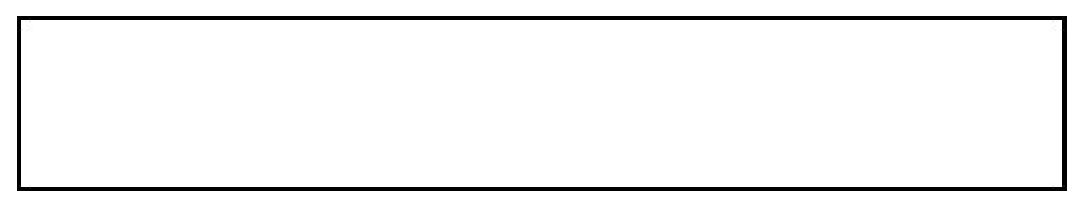
\includegraphics[width=0.9\textwidth]{fig.eps}
% \caption{This is a widefig. This is an example of long caption this is an example of long caption  this is an example of long caption this is an example of long caption}\label{fig1}
% \end{figure}

% In case of double column layout, the above format puts figure captions/images to single column width. To get spanned images, we need to provide \verb+\begin{figure*}+ \verb+...+ \verb+\end{figure*}+.

% For sample purpose, we have included the width of images in the optional argument of \verb+\includegraphics+ tag. Please ignore this. 

% \section{Algorithms, Program codes and Listings}\label{sec7}

% Packages \verb+algorithm+, \verb+algorithmicx+ and \verb+algpseudocode+ are used for setting algorithms in \LaTeX\ using the format:

% %%=============================================%%
% %% For presentation purpose, we have included  %%
% %% \bigskip command. Please ignore this.       %%
% %%=============================================%%
% \bigskip
% \begin{verbatim}
% \begin{algorithm}
% \caption{<alg-caption>}\label{<alg-label>}
% \begin{algorithmic}[1]
% . . .
% \end{algorithmic}
% \end{algorithm}
% \end{verbatim}
% \bigskip
% %%=============================================%%
% %% For presentation purpose, we have included  %%
% %% \bigskip command. Please ignore this.       %%
% %%=============================================%%

% You may refer above listed package documentations for more details before setting \verb+algorithm+ environment. For program codes, the ``verbatim'' package is required and the command to be used is \verb+\begin{verbatim}+ \verb+...+ \verb+\end{verbatim}+. 

% Similarly, for \verb+listings+, use the \verb+listings+ package. \verb+\begin{lstlisting}+ \verb+...+ \verb+\end{lstlisting}+ is used to set environments similar to \verb+verbatim+ environment. Refer to the \verb+lstlisting+ package documentation for more details.

% A fast exponentiation procedure:

% \lstset{texcl=true,basicstyle=\small\sf,commentstyle=\small\rm,mathescape=true,escapeinside={(*}{*)}}
% \begin{lstlisting}
% begin
%   for $i:=1$ to $10$ step $1$ do
%       expt($2,i$);  
%       newline() od                (*\textrm{Comments will be set flush to the right margin}*)
% where
% proc expt($x,n$) $\equiv$
%   $z:=1$;
%   do if $n=0$ then exit fi;
%      do if odd($n$) then exit fi;                 
%         comment: (*\textrm{This is a comment statement;}*)
%         $n:=n/2$; $x:=x*x$ od;
%      { $n>0$ };
%      $n:=n-1$; $z:=z*x$ od;
%   print($z$). 
% end
% \end{lstlisting}

% \begin{algorithm}
% \caption{Calculate $y = x^n$}\label{algo1}
% \begin{algorithmic}[1]
% \Require $n \geq 0 \vee x \neq 0$
% \Ensure $y = x^n$ 
% \State $y \Leftarrow 1$
% \If{$n < 0$}\label{algln2}
%         \State $X \Leftarrow 1 / x$
%         \State $N \Leftarrow -n$
% \Else
%         \State $X \Leftarrow x$
%         \State $N \Leftarrow n$
% \EndIf
% \While{$N \neq 0$}
%         \If{$N$ is even}
%             \State $X \Leftarrow X \times X$
%             \State $N \Leftarrow N / 2$
%         \Else[$N$ is odd]
%             \State $y \Leftarrow y \times X$
%             \State $N \Leftarrow N - 1$
%         \EndIf
% \EndWhile
% \end{algorithmic}
% \end{algorithm}

% %%=============================================%%
% %% For presentation purpose, we have included  %%
% %% \bigskip command. Please ignore this.       %%
% %%=============================================%%
% \bigskip
% \begin{minipage}{\hsize}%
% \lstset{frame=single,framexleftmargin=-1pt,framexrightmargin=-17pt,framesep=12pt,linewidth=0.98\textwidth,language=pascal}% Set your language (you can change the language for each code-block optionally)
% %%% Start your code-block
% \begin{lstlisting}
% for i:=maxint to 0 do
% begin
% { do nothing }
% end;
% Write('Case insensitive ');
% Write('Pascal keywords.');
% \end{lstlisting}
% \end{minipage}

% \section{Cross referencing}\label{sec8}

% Environments such as figure, table, equation and align can have a label
% declared via the \verb+\label{#label}+ command. For figures and table
% environments use the \verb+\label{}+ command inside or just
% below the \verb+\caption{}+ command. You can then use the
% \verb+\ref{#label}+ command to cross-reference them. As an example, consider
% the label declared for Figure~\ref{fig1} which is
% \verb+\label{fig1}+. To cross-reference it, use the command 
% \verb+Figure \ref{fig1}+, for which it comes up as
% ``Figure~\ref{fig1}''. 

% To reference line numbers in an algorithm, consider the label declared for the line number 2 of Algorithm~\ref{algo1} is \verb+\label{algln2}+. To cross-reference it, use the command \verb+\ref{algln2}+ for which it comes up as line~\ref{algln2} of Algorithm~\ref{algo1}.

% \subsection{Details on reference citations}\label{subsec7}

% Standard \LaTeX\ permits only numerical citations. To support both numerical and author-year citations this template uses \verb+natbib+ \LaTeX\ package. For style guidance please refer to the template user manual.

% Here is an example for \verb+\cite{...}+: \cite{bib1}. Another example for \verb+\citep{...}+: \citep{bib2}. For author-year citation mode, \verb+\cite{...}+ prints Jones et al. (1990) and \verb+\citep{...}+ prints (Jones et al., 1990).

% All cited bib entries are printed at the end of this article: \cite{bib3}, \cite{bib4}, \cite{bib5}, \cite{bib6}, \cite{bib7}, \cite{bib8}, \cite{bib9}, \cite{bib10}, \cite{bib11}, \cite{bib12} and \cite{bib13}.

% \section{Examples for theorem like environments}\label{sec10}

% For theorem like environments, we require \verb+amsthm+ package. There are three types of predefined theorem styles exists---\verb+thmstyleone+, \verb+thmstyletwo+ and \verb+thmstylethree+ 

% %%=============================================%%
% %% For presentation purpose, we have included  %%
% %% \bigskip command. Please ignore this.       %%
% %%=============================================%%
% \bigskip
% \begin{tabular}{|l|p{19pc}|}
% \hline
% \verb+thmstyleone+ & Numbered, theorem head in bold font and theorem text in italic style \\\hline
% \verb+thmstyletwo+ & Numbered, theorem head in roman font and theorem text in italic style \\\hline
% \verb+thmstylethree+ & Numbered, theorem head in bold font and theorem text in roman style \\\hline
% \end{tabular}
% \bigskip
% %%=============================================%%
% %% For presentation purpose, we have included  %%
% %% \bigskip command. Please ignore this.       %%
% %%=============================================%%

% For mathematics journals, theorem styles can be included as shown in the following examples:

% \begin{theorem}[Theorem subhead]\label{thm1}
% Example theorem text. Example theorem text. Example theorem text. Example theorem text. Example theorem text. 
% Example theorem text. Example theorem text. Example theorem text. Example theorem text. Example theorem text. 
% Example theorem text. 
% \end{theorem}

% Sample body text. Sample body text. Sample body text. Sample body text. Sample body text. Sample body text. Sample body text. Sample body text.

% \begin{proposition}
% Example proposition text. Example proposition text. Example proposition text. Example proposition text. Example proposition text. 
% Example proposition text. Example proposition text. Example proposition text. Example proposition text. Example proposition text. 
% \end{proposition}

% Sample body text. Sample body text. Sample body text. Sample body text. Sample body text. Sample body text. Sample body text. Sample body text.

% \begin{example}
% Phasellus adipiscing semper elit. Proin fermentum massa
% ac quam. Sed diam turpis, molestie vitae, placerat a, molestie nec, leo. Maecenas lacinia. Nam ipsum ligula, eleifend
% at, accumsan nec, suscipit a, ipsum. Morbi blandit ligula feugiat magna. Nunc eleifend consequat lorem. 
% \end{example}

% Sample body text. Sample body text. Sample body text. Sample body text. Sample body text. Sample body text. Sample body text. Sample body text.

% \begin{remark}
% Phasellus adipiscing semper elit. Proin fermentum massa
% ac quam. Sed diam turpis, molestie vitae, placerat a, molestie nec, leo. Maecenas lacinia. Nam ipsum ligula, eleifend
% at, accumsan nec, suscipit a, ipsum. Morbi blandit ligula feugiat magna. Nunc eleifend consequat lorem. 
% \end{remark}

% Sample body text. Sample body text. Sample body text. Sample body text. Sample body text. Sample body text. Sample body text. Sample body text.

% \begin{definition}[Definition sub head]
% Example definition text. Example definition text. Example definition text. Example definition text. Example definition text. Example definition text. Example definition text. Example definition text. 
% \end{definition}

% Additionally a predefined ``proof'' environment is available: \verb+\begin{proof}+ \verb+...+ \verb+\end{proof}+. This prints a ``Proof'' head in italic font style and the ``body text'' in roman font style with an open square at the end of each proof environment. 

% \begin{proof}
% Example for proof text. Example for proof text. Example for proof text. Example for proof text. Example for proof text. Example for proof text. Example for proof text. Example for proof text. Example for proof text. Example for proof text. 
% \end{proof}

% Sample body text. Sample body text. Sample body text. Sample body text. Sample body text. Sample body text. Sample body text. Sample body text.

% \begin{proof}[Proof of Theorem~{\upshape\ref{thm1}}]
% Example for proof text. Example for proof text. Example for proof text. Example for proof text. Example for proof text. Example for proof text. Example for proof text. Example for proof text. Example for proof text. Example for proof text. 
% \end{proof}

% \noindent
% For a quote environment, use \verb+\begin{quote}...\end{quote}+
% \begin{quote}
% Quoted text example. Aliquam porttitor quam a lacus. Praesent vel arcu ut tortor cursus volutpat. In vitae pede quis diam bibendum placerat. Fusce elementum
% convallis neque. Sed dolor orci, scelerisque ac, dapibus nec, ultricies ut, mi. Duis nec dui quis leo sagittis commodo.
% \end{quote}

% Sample body text. Sample body text. Sample body text. Sample body text. Sample body text (refer Figure~\ref{fig1}). Sample body text. Sample body text. Sample body text (refer Table~\ref{tab3}). 

\section{Methods}\label{sec11}

The methodology of this study centres on two distinct feature-extraction pipelines applied to neonatal EEG recordings. The first pipeline derives compact spectral descriptors by fitting a linear model to the log-transformed power spectral density (PSD) within each of the classical neurophysiological frequency bands. This parameterisation strategy---characterising a spectrum by its slope, midband-fit value, and intercept---has been validated in an entirely different biomedical domain: Sinha et al.\ demonstrated that the same trio of spectral parameters, extracted from multiwavelength photoacoustic signals, could reliably distinguish malignant prostate tissue from benign and normal specimens in an ex-vivo setting \cite{sinha2016}. Their success in a non-neural context motivates the hypothesis that these frequency-domain descriptors capture fundamental properties of spectral shape that generalise across signal modalities. The second pipeline employs Empirical Mode Decomposition (EMD) to decompose each EEG epoch into data-driven oscillatory components, from which energy- and frequency-based statistics are computed. Both feature sets are subsequently reduced to a common dimensionality via Principal Component Analysis and classified by an identical feedforward neural network, ensuring that any performance difference reflects the quality of the underlying features rather than architectural bias.

\subsection{Dataset}\label{subsec:dataset}

This study utilised a publicly available neonatal EEG corpus recorded at Helsinki University Hospital. The cohort comprised 79 neonates, of whom 39 had seizures confirmed through expert consensus annotation, while the remaining 40 served as non-seizure controls. Continuous multi-channel EEG was acquired for each infant, with recording durations spanning approximately one hour per subject (median 74 minutes; interquartile range 64--96 minutes). Seizure events were independently annotated by three qualified clinical neurophysiologists; only epochs receiving unanimous agreement from all three annotators were retained as seizure ground truth, and any epochs with partial or conflicting annotations were excluded from the analysis to minimise label noise. Annotations were exported at one-second temporal resolution, specifying onset time and duration but omitting spatial localisation or electrographic seizure type due to the export format.

To match the montage employed during the original annotation process, the raw referential recordings were re-referenced offline to an anterior--posterior bipolar configuration. This step ensured consistency between the derivations seen by the annotators and the signals presented to the automated pipeline, thereby guarding against artefactual discrepancies that could arise from montage mismatch.

\subsection{Log-transformed Power Spectral Density and Curve Fitting}\label{subsec:psd}

Power spectral density quantifies how the energy of a signal is distributed across frequency, providing a compact summary of its oscillatory content. Because neurophysiological activity is conventionally partitioned into distinct frequency bands---each associated with different brain states and pathological signatures---the EEG signal was first pre-processed with a fourth-order Butterworth bandpass filter configured to isolate successive frequency ranges. Four standard bands were considered: delta (0.7--4~Hz), theta (4--8~Hz), alpha (8--13~Hz), and beta (13--30~Hz). Filtering each band independently yielded cleaner spectral estimates within the neurologically relevant ranges and suppressed out-of-band noise that could otherwise distort the subsequent analysis.

For each filtered band and epoch, the power spectral density was estimated and converted to a logarithmic (decibel) scale. This transformation compresses the large dynamic range typical of EEG power spectra while linearising the characteristic $1/f^{-\alpha}$ decay, making it amenable to simple parametric modelling. A least-squares linear regression was then fitted to the log-power versus log-frequency curve within each band, producing a straight line that captures the dominant spectral trend of that band.

From this fitted line, three scalar parameters were extracted per band: the \emph{slope}, quantifying the rate of spectral roll-off; the \emph{midband-fit} value, representing the predicted log-power at the geometric centre of the band; and the \emph{intercept}, indicating the baseline log-power level. This parameterisation directly follows the framework demonstrated by Sinha et al.\ in their photoacoustic tissue-classification study \cite{sinha2016}, where the same three spectral descriptors---slope, midband fit, and intercept---proved effective for differentiating malignant from benign and normal prostate tissue on the basis of frequency-domain signatures alone. By applying this proven spectral characterisation to neonatal EEG, the present work tests whether the same compact set of parameters can capture the spectral changes that distinguish seizure from non-seizure brain activity. With four frequency bands and three parameters per band, the full feature vector for each epoch consisted of twelve elements.

\subsection{Empirical Mode Decomposition Feature Set}\label{subsec:emd}

As a complementary, data-driven alternative to the spectral-fitting approach, Empirical Mode Decomposition (EMD) was employed to decompose each EEG epoch into a set of oscillatory components known as Intrinsic Mode Functions (IMFs). Unlike Fourier-based methods, which project the signal onto fixed sinusoidal bases, EMD adapts entirely to the local characteristics of the data, making it particularly suited to non-stationary signals such as neonatal EEG.

The decomposition proceeds through an iterative sifting procedure. In each iteration, the local maxima and minima of the signal are identified and connected by cubic-spline interpolation to form upper and lower envelopes, respectively. The mean of these envelopes is subtracted from the signal, and the process repeats until the residual satisfies the narrow-band criterion defining a valid IMF---namely, that the number of extrema and zero crossings differs by at most one, and that the local mean of the envelopes is approximately zero. Once an IMF is extracted, the procedure is applied to the remainder, yielding successive components of decreasing characteristic frequency until the residual becomes monotonic.

To maintain a uniform feature-vector length across all epochs, only a fixed number of the leading IMFs were retained for analysis. From each retained IMF, four summary statistics were computed: the log-transformed energy, the mean instantaneous frequency obtained via the Hilbert analytic signal, the standard deviation of the instantaneous amplitude envelope, and the spectral entropy of the IMF's own power spectrum. These per-IMF descriptors were concatenated into a single feature vector per epoch, providing a compact yet informative representation of the signal's intrinsic oscillatory structure for downstream classification.

\subsection{Evaluation}\label{subsec:evaluation}

\subsubsection{Dimensionality Reduction and Statistical Testing}

Principal Component Analysis (PCA) was applied independently to each feature set to project both pipelines into a comparable, lower-dimensional space. This step removed redundant or correlated feature dimensions while retaining the principal variance-bearing components, ensuring that the subsequent classifier operated on representations of equivalent complexity regardless of the original feature-set size.

To quantify the discriminative relevance of individual principal components, independent-samples Welch t-tests were conducted between the seizure and non-seizure groups for each component. The resulting t-statistics and associated p-values provided a transparent, interpretable assessment of which spectral or EMD-derived dimensions carried the greatest group-separability signal, complementing the opaque decision boundaries of the neural network classifier.

\subsubsection{Classification Architecture}

An identical feedforward artificial neural network was used for both pipelines to ensure that any performance difference could be attributed to the feature representations rather than the classifier. The architecture consisted of three fully connected hidden layers with 128, 64, and 32 units, respectively. Each hidden layer was followed by batch normalisation to stabilise internal activations, a Rectified Linear Unit (ReLU) activation function to introduce non-linearity, and a dropout layer with a retention probability of 0.7 to mitigate overfitting. The output layer comprised a single unit with a softmax activation producing class-posterior probabilities for the seizure and non-seizure states.

Training minimised the categorical cross-entropy loss with inverse-frequency class weights to counteract the severe imbalance between seizure and non-seizure epochs. The Adam optimiser was employed with a fixed learning rate of $1 \times 10^{-3}$ and a batch size of 64 samples. An early-stopping criterion monitored validation loss over a patience window of 10--25 epochs, halting training whenever no improvement was observed, with a hard cap of 100 epochs.

\subsubsection{Post-processing and Threshold Optimisation}

The raw softmax probabilities were smoothed with a causal moving-average filter to attenuate transient fluctuations and produce a temporally coherent probability trajectory. This step suppressed isolated spikes and brief disturbances that did not correspond to sustained electrographic activity. An optimal decision threshold was then determined on the validation set to maximise a chosen performance metric, converting the smoothed probability into a binary seizure/non-seizure classification.

\subsubsection{Class-Imbalance Management}

Neonatal EEG recordings are characterised by extreme class imbalance, with non-seizure epochs vastly outnumbering seizure epochs. To address this, an adaptive nearest-neighbour downsampling strategy was employed. All seizure epochs were retained in full, ensuring complete coverage of the positive class. Each non-seizure epoch was then scored according to its temporal proximity to the nearest seizure event, producing a ranking that prioritised boundary-adjacent non-seizure samples. The closest non-seizure epochs were selected according to a configurable target ratio (default 2.0), subject to a minimum-ratio safeguard guaranteeing that the non-seizure class always exceeded the seizure class in absolute count. This strategy reduced the magnitude of the imbalance while preserving the temporal context surrounding seizure transitions, which is important for the classifier to learn discriminative boundary features.



% Topical subheadings are allowed. Authors must ensure that their Methods section includes adequate experimental and characterization data necessary for others in the field to reproduce their work. Authors are encouraged to include RIIDs where appropriate. 

% \textbf{Ethical approval declarations} (only required where applicable) Any article reporting experiment/s carried out on (i)~live vertebrate (or higher invertebrates), (ii)~humans or (iii)~human samples must include an unambiguous statement within the methods section that meets the following requirements: 

% \begin{enumerate}[1.]
% \item Approval: a statement which confirms that all experimental protocols were approved by a named institutional and/or licensing committee. Please identify the approving body in the methods section

% \item Accordance: a statement explicitly saying that the methods were carried out in accordance with the relevant guidelines and regulations

% \item Informed consent (for experiments involving humans or human tissue samples): include a statement confirming that informed consent was obtained from all participants and/or their legal guardian/s
% \end{enumerate}

% If your manuscript includes potentially identifying patient/participant information, or if it describes human transplantation research, or if it reports results of a clinical trial then  additional information will be required. Please visit (\url{https://www.nature.com/nature-research/editorial-policies}) for Nature Portfolio journals, (\url{https://www.springer.com/gp/authors-editors/journal-author/journal-author-helpdesk/publishing-ethics/14214}) for Springer Nature journals, or (\url{https://www.biomedcentral.com/getpublished/editorial-policies\#ethics+and+consent}) for BMC.
\section{Results}

To assess the discriminative relevance of individual feature components, independent-samples t-tests were conducted between seizure and non-seizure groups for each principal component. Figures~\ref{fig:freq_t_stat} and~\ref{fig:freq_significance} display the t-statistics and corresponding negative log-transformed p-values for the frequency-domain features, while Figures~\ref{fig:emd_t_stat} and~\ref{fig:emd_significance} present the analogous results for the EMD features.

\begin{figure}[h!]
    \centering
    % FREQ SIDE BY SIDE
    \begin{subfigure}{0.7\linewidth}
        \centering
        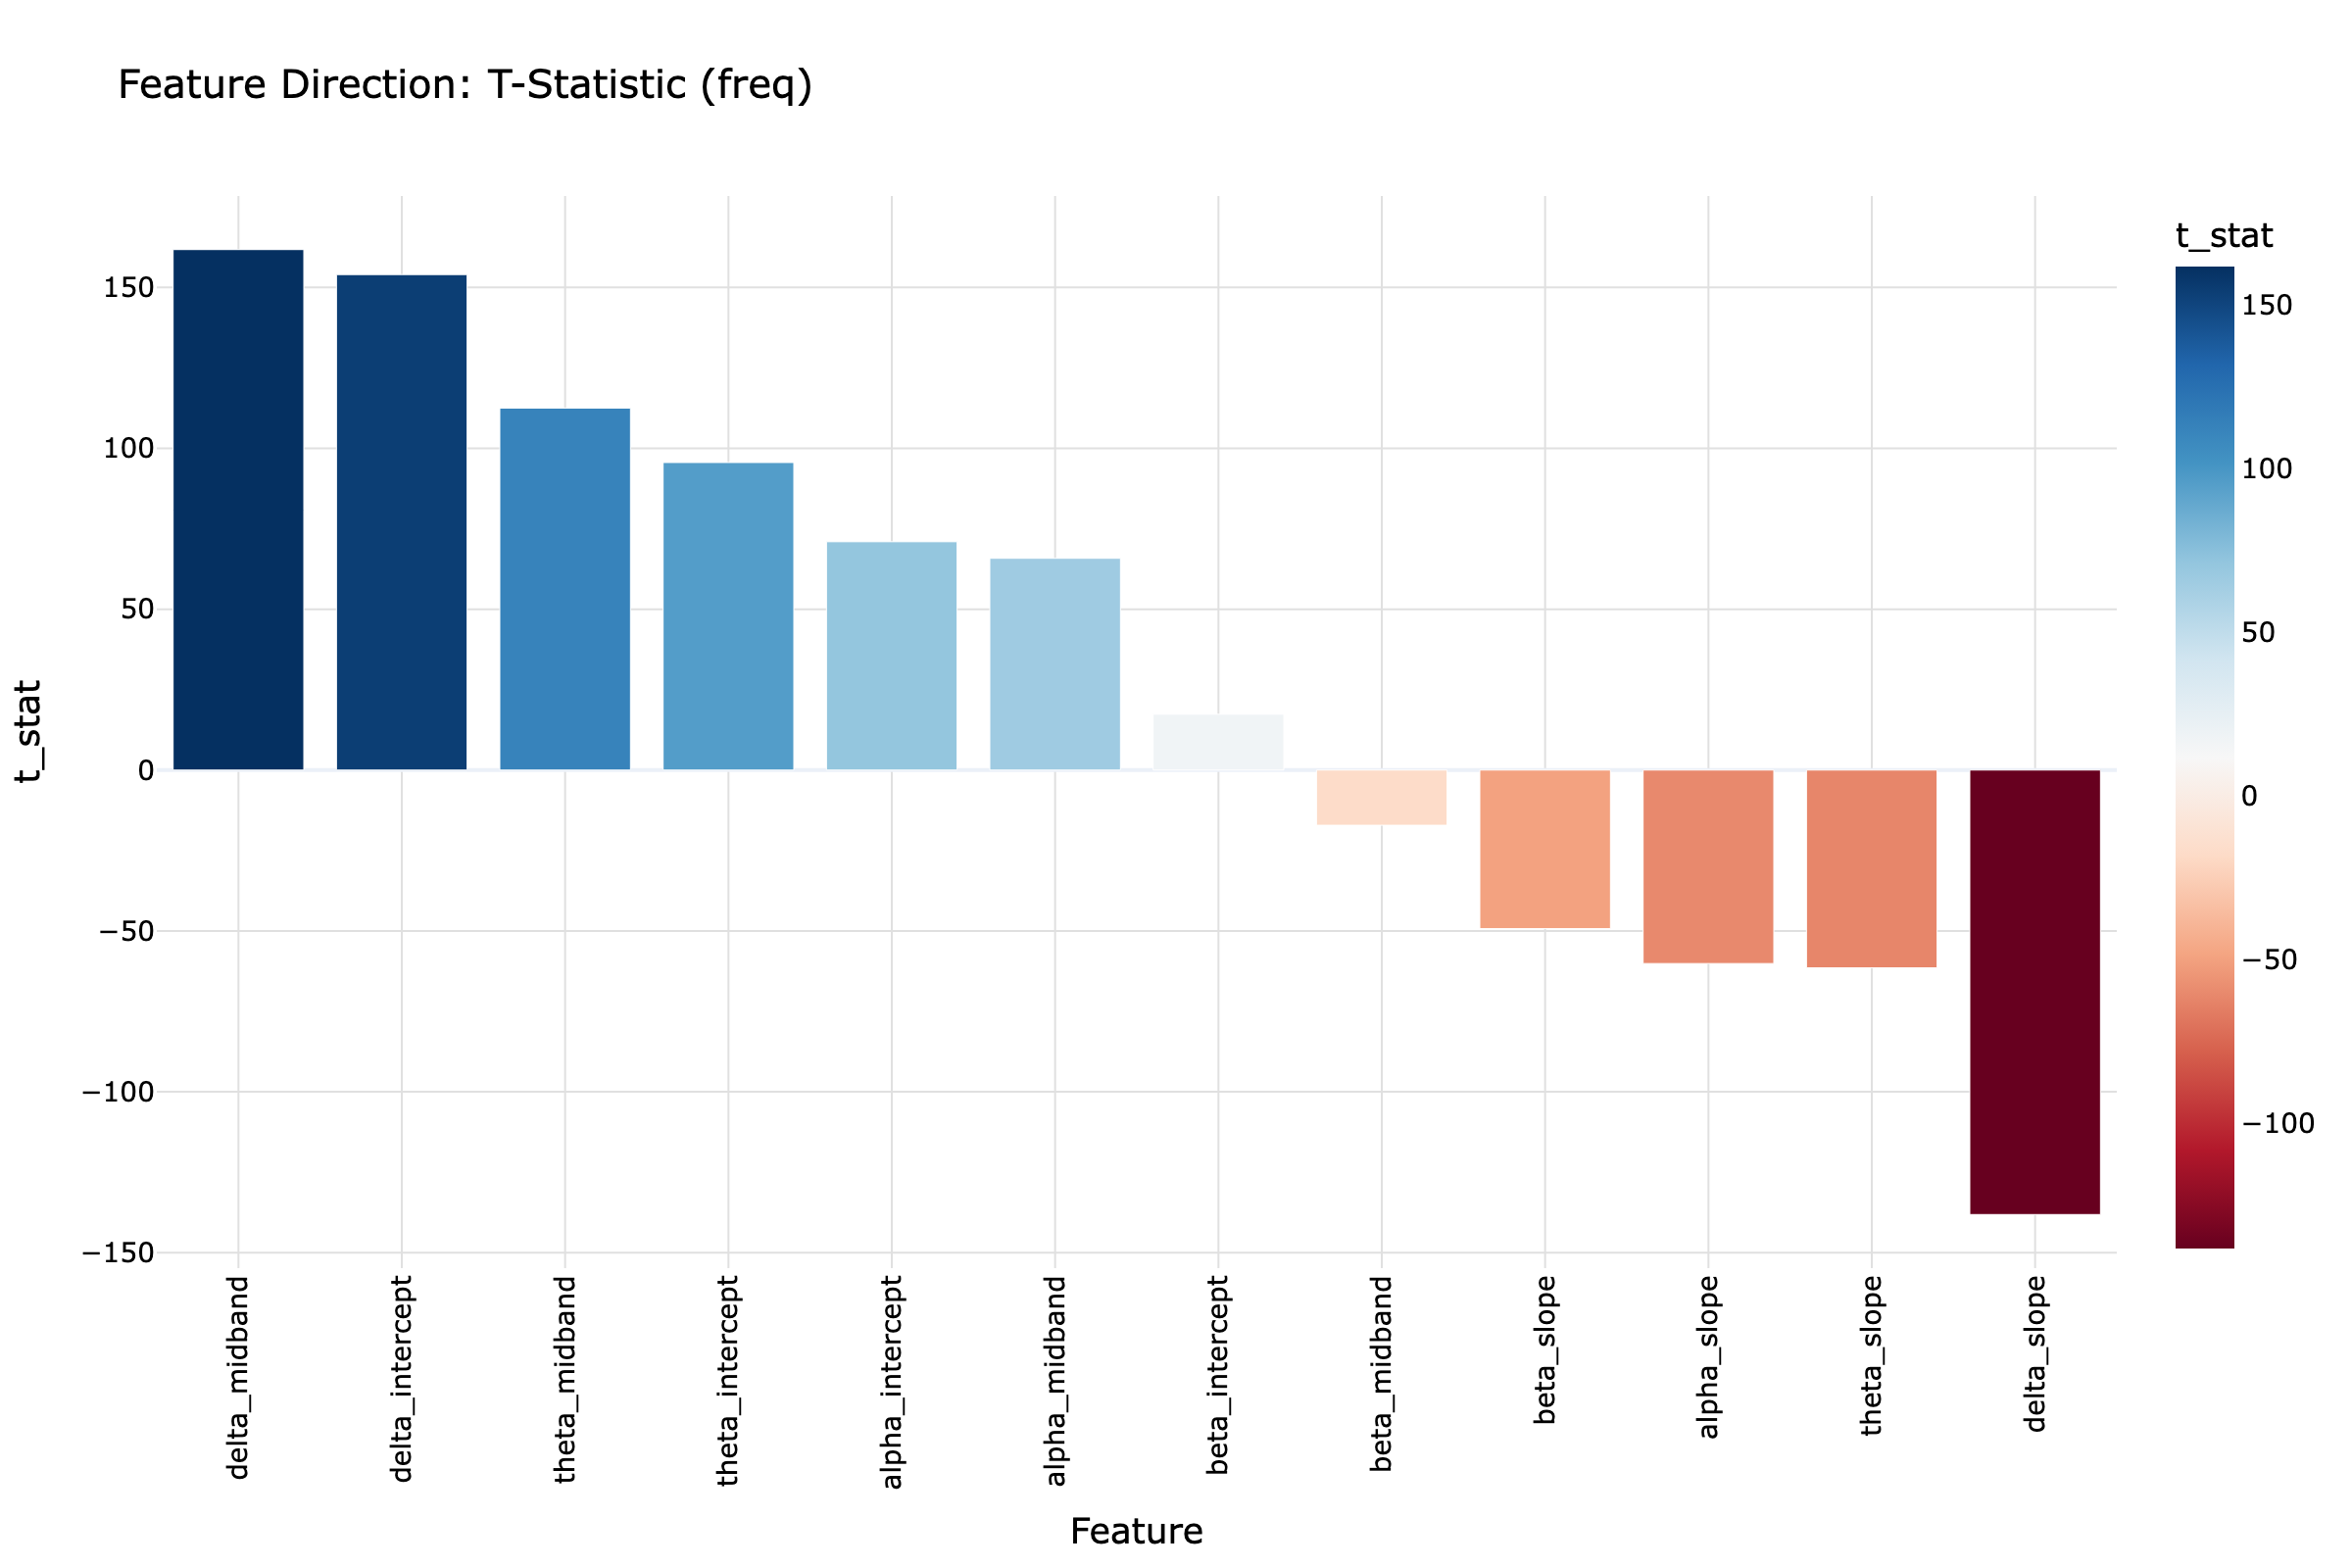
\includegraphics[width=\linewidth]{public/freq_t_stat.png}
        \caption{Frequency features: t-statistic per principal component}
        \label{fig:freq_t_stat}
    \end{subfigure}
    \hfill
    \begin{subfigure}{0.7\linewidth}
        \centering
        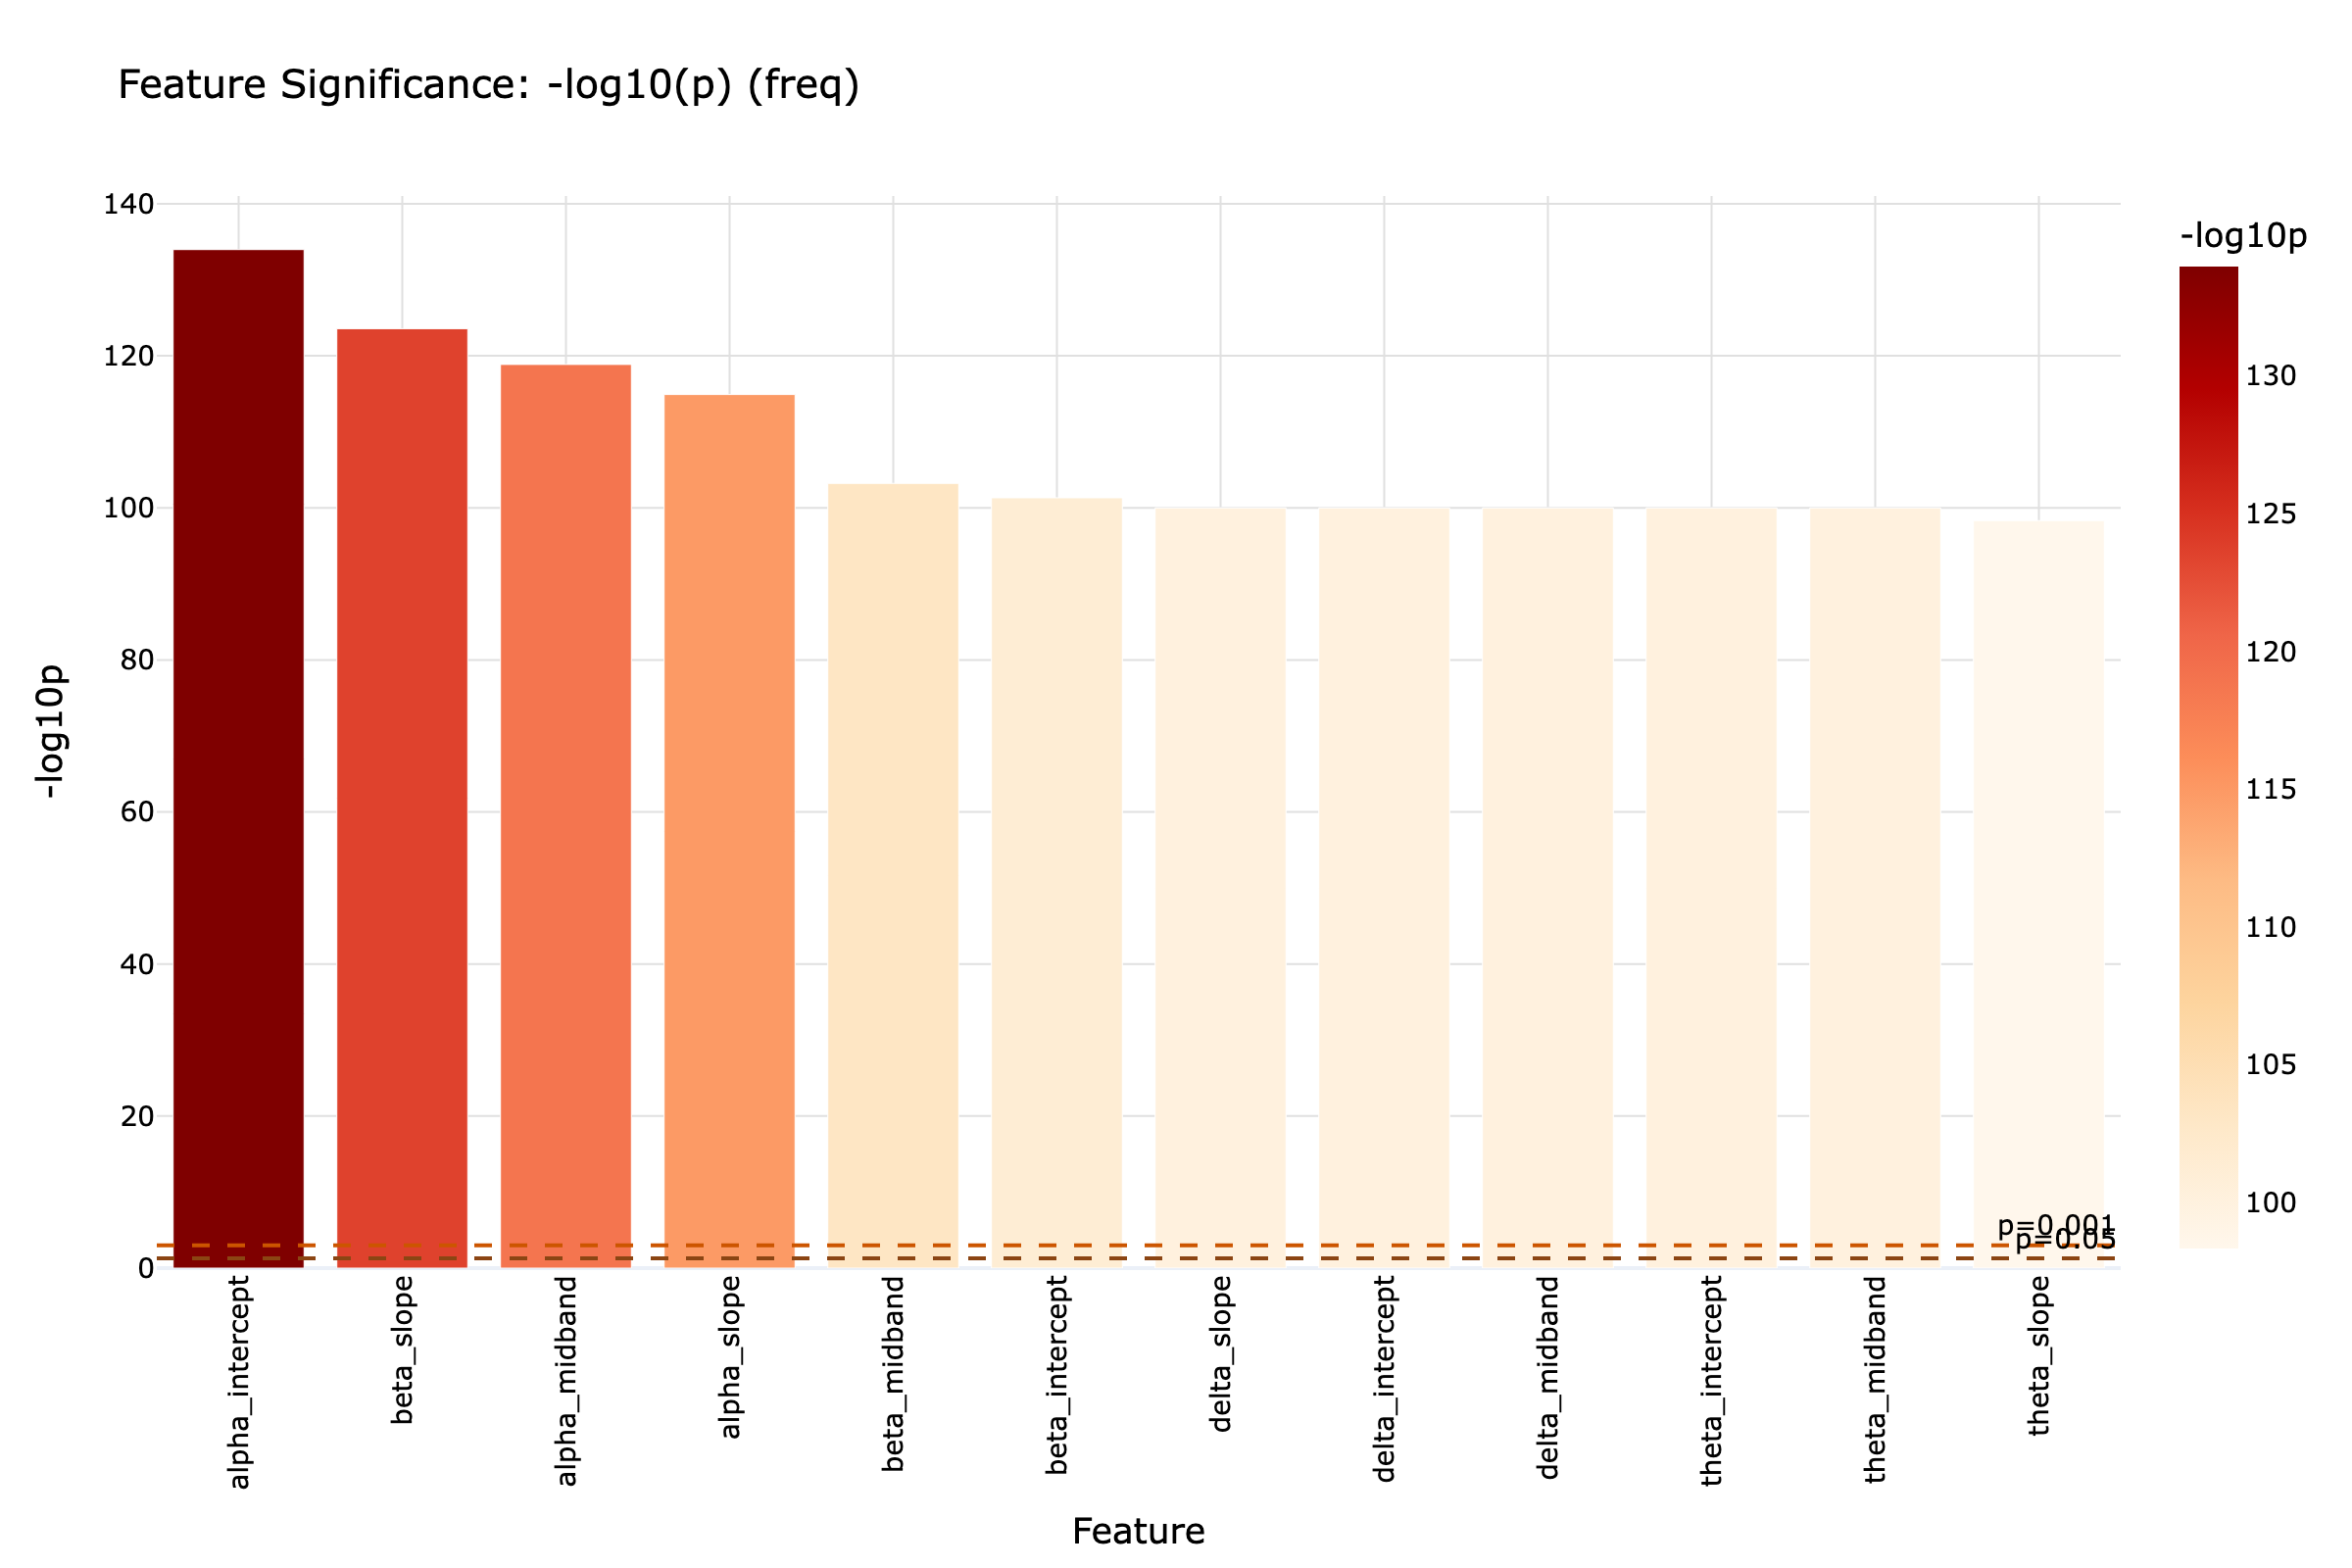
\includegraphics[width=\linewidth]{public/freq_significance.png}
        \caption{Frequency features: $-\log(p)$ per principal component}
        \label{fig:freq_significance}
    \end{subfigure}
    \caption{Statistical comparison of PCA-reduced frequency-domain features between seizure and non-seizure epochs.}
\end{figure}

\begin{figure}[h!]
    \centering
    % EMD SIDE BY SIDE
    \begin{subfigure}{0.7\linewidth}
        \centering
        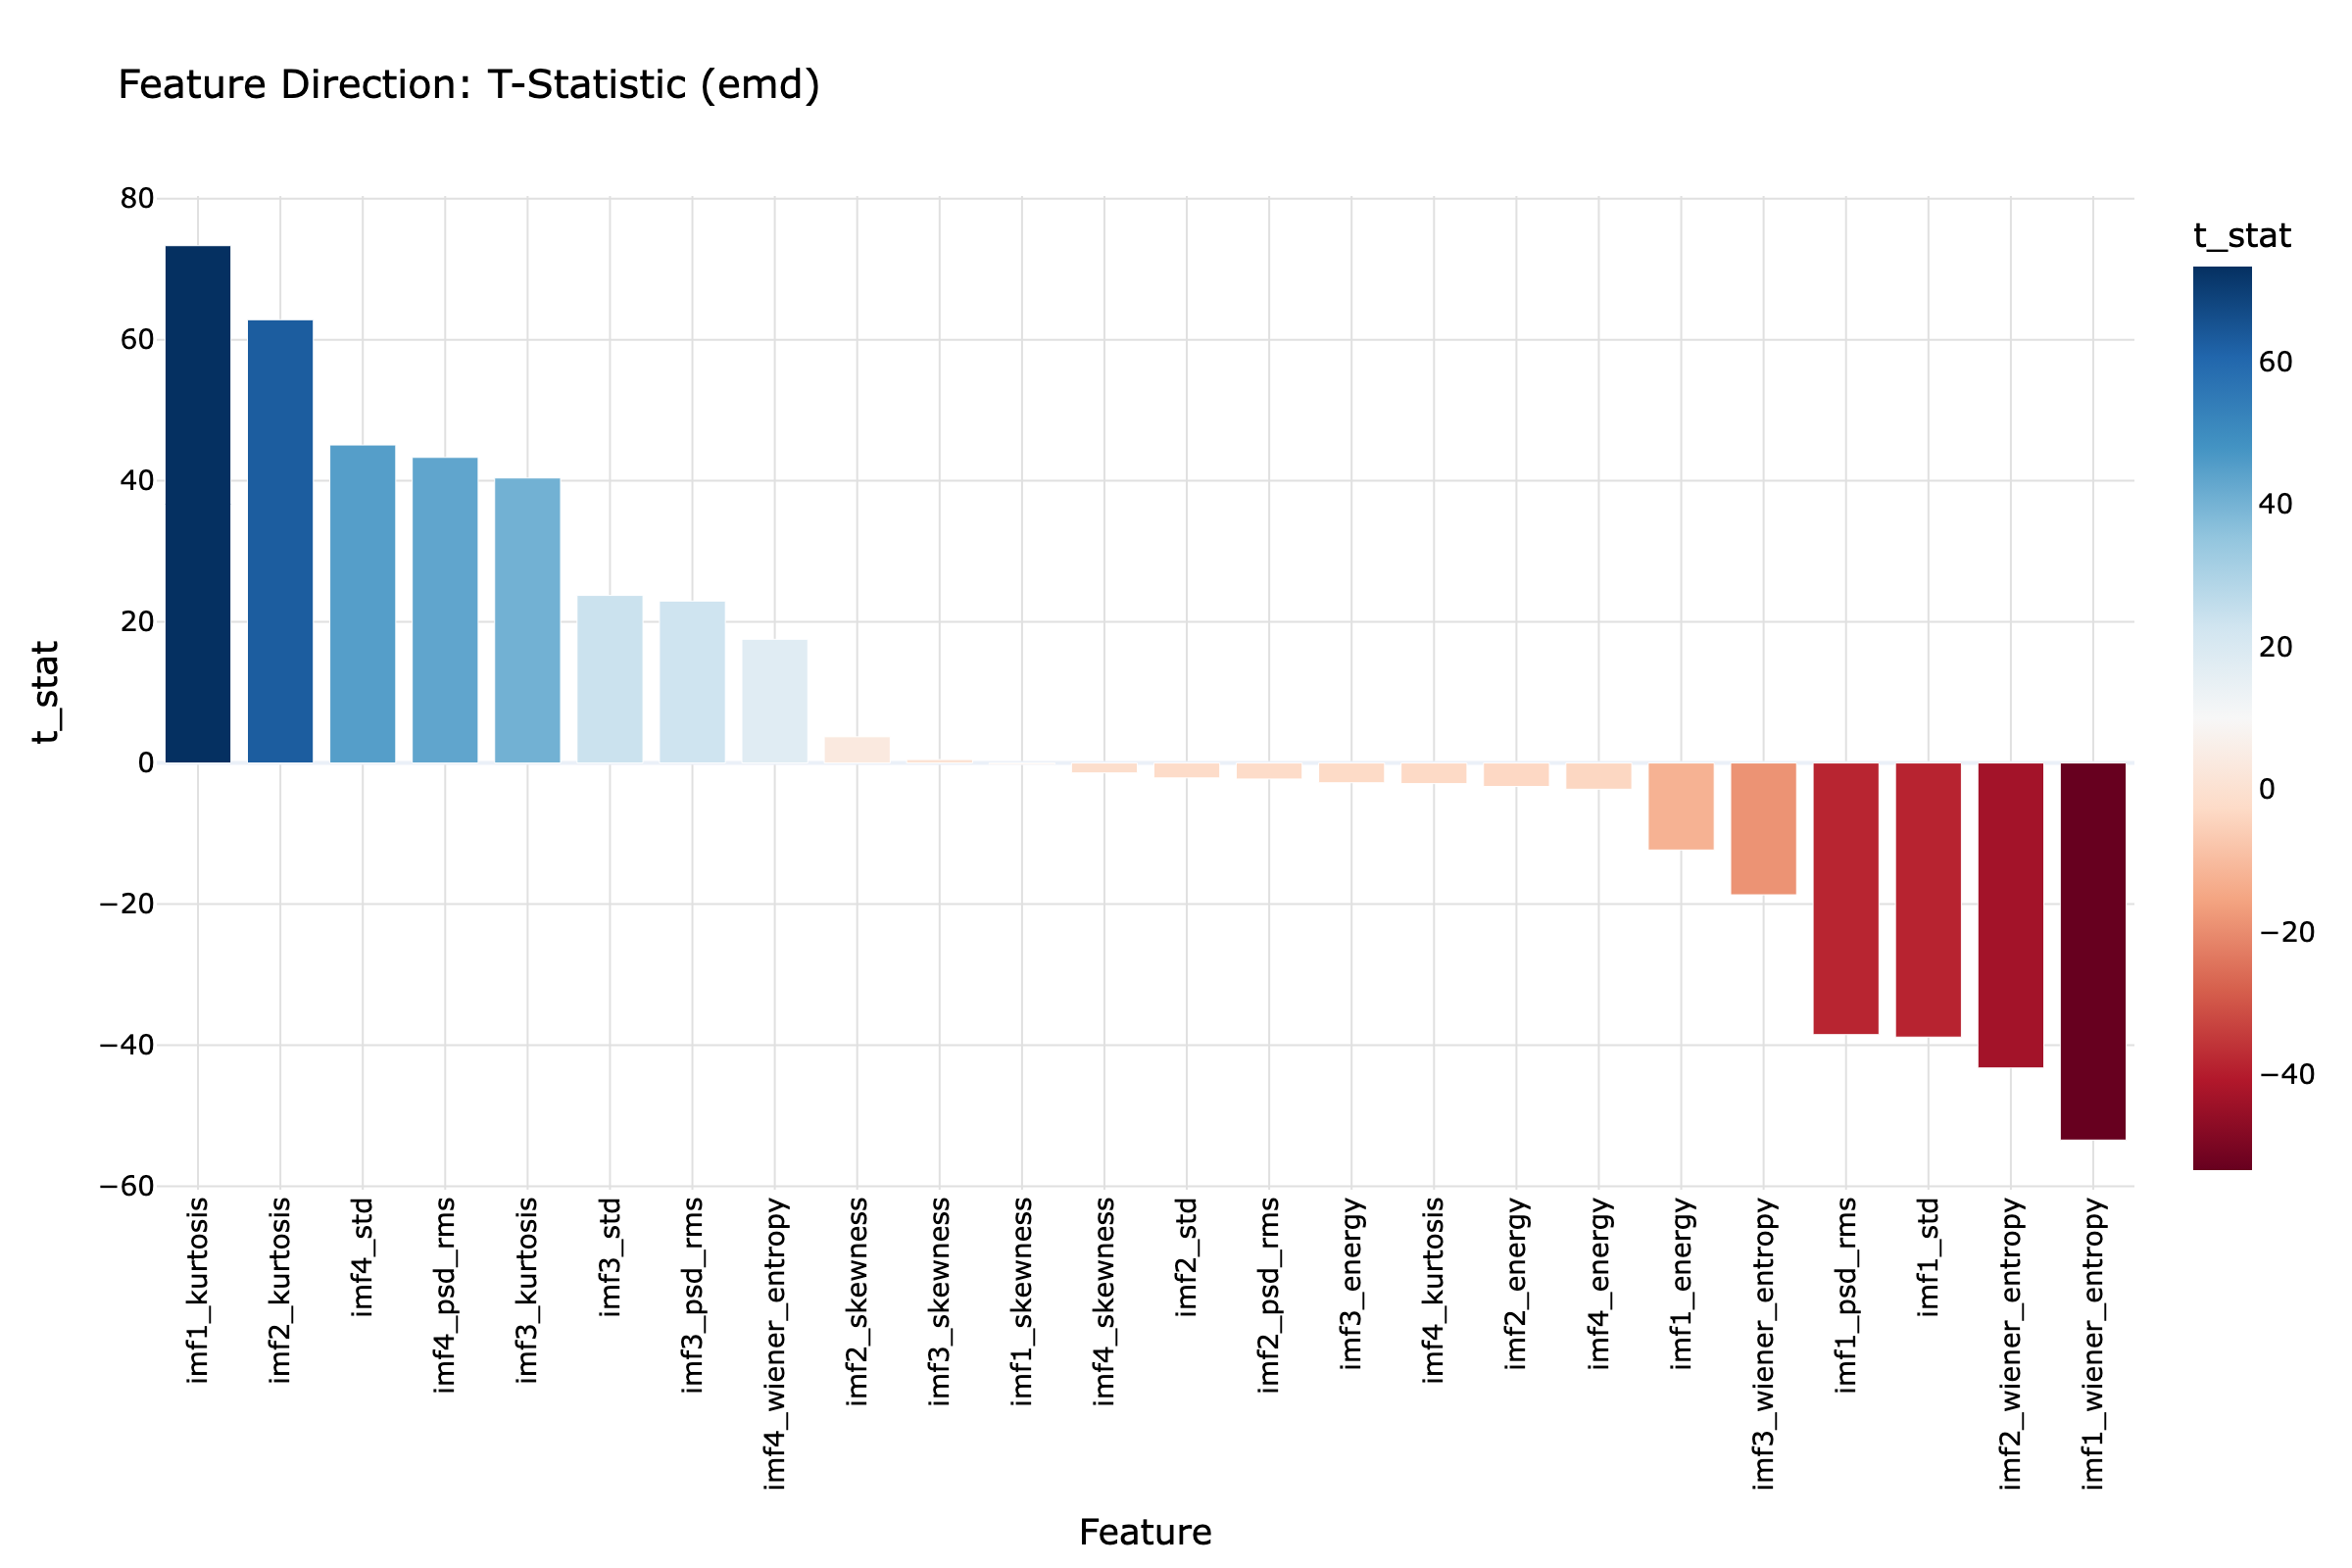
\includegraphics[width=\linewidth]{public/emd_t_stat.png}
        \caption{EMD features: t-statistic per principal component}
        \label{fig:emd_t_stat}
    \end{subfigure}
    \hfill
    \begin{subfigure}{0.7\linewidth}
        \centering
        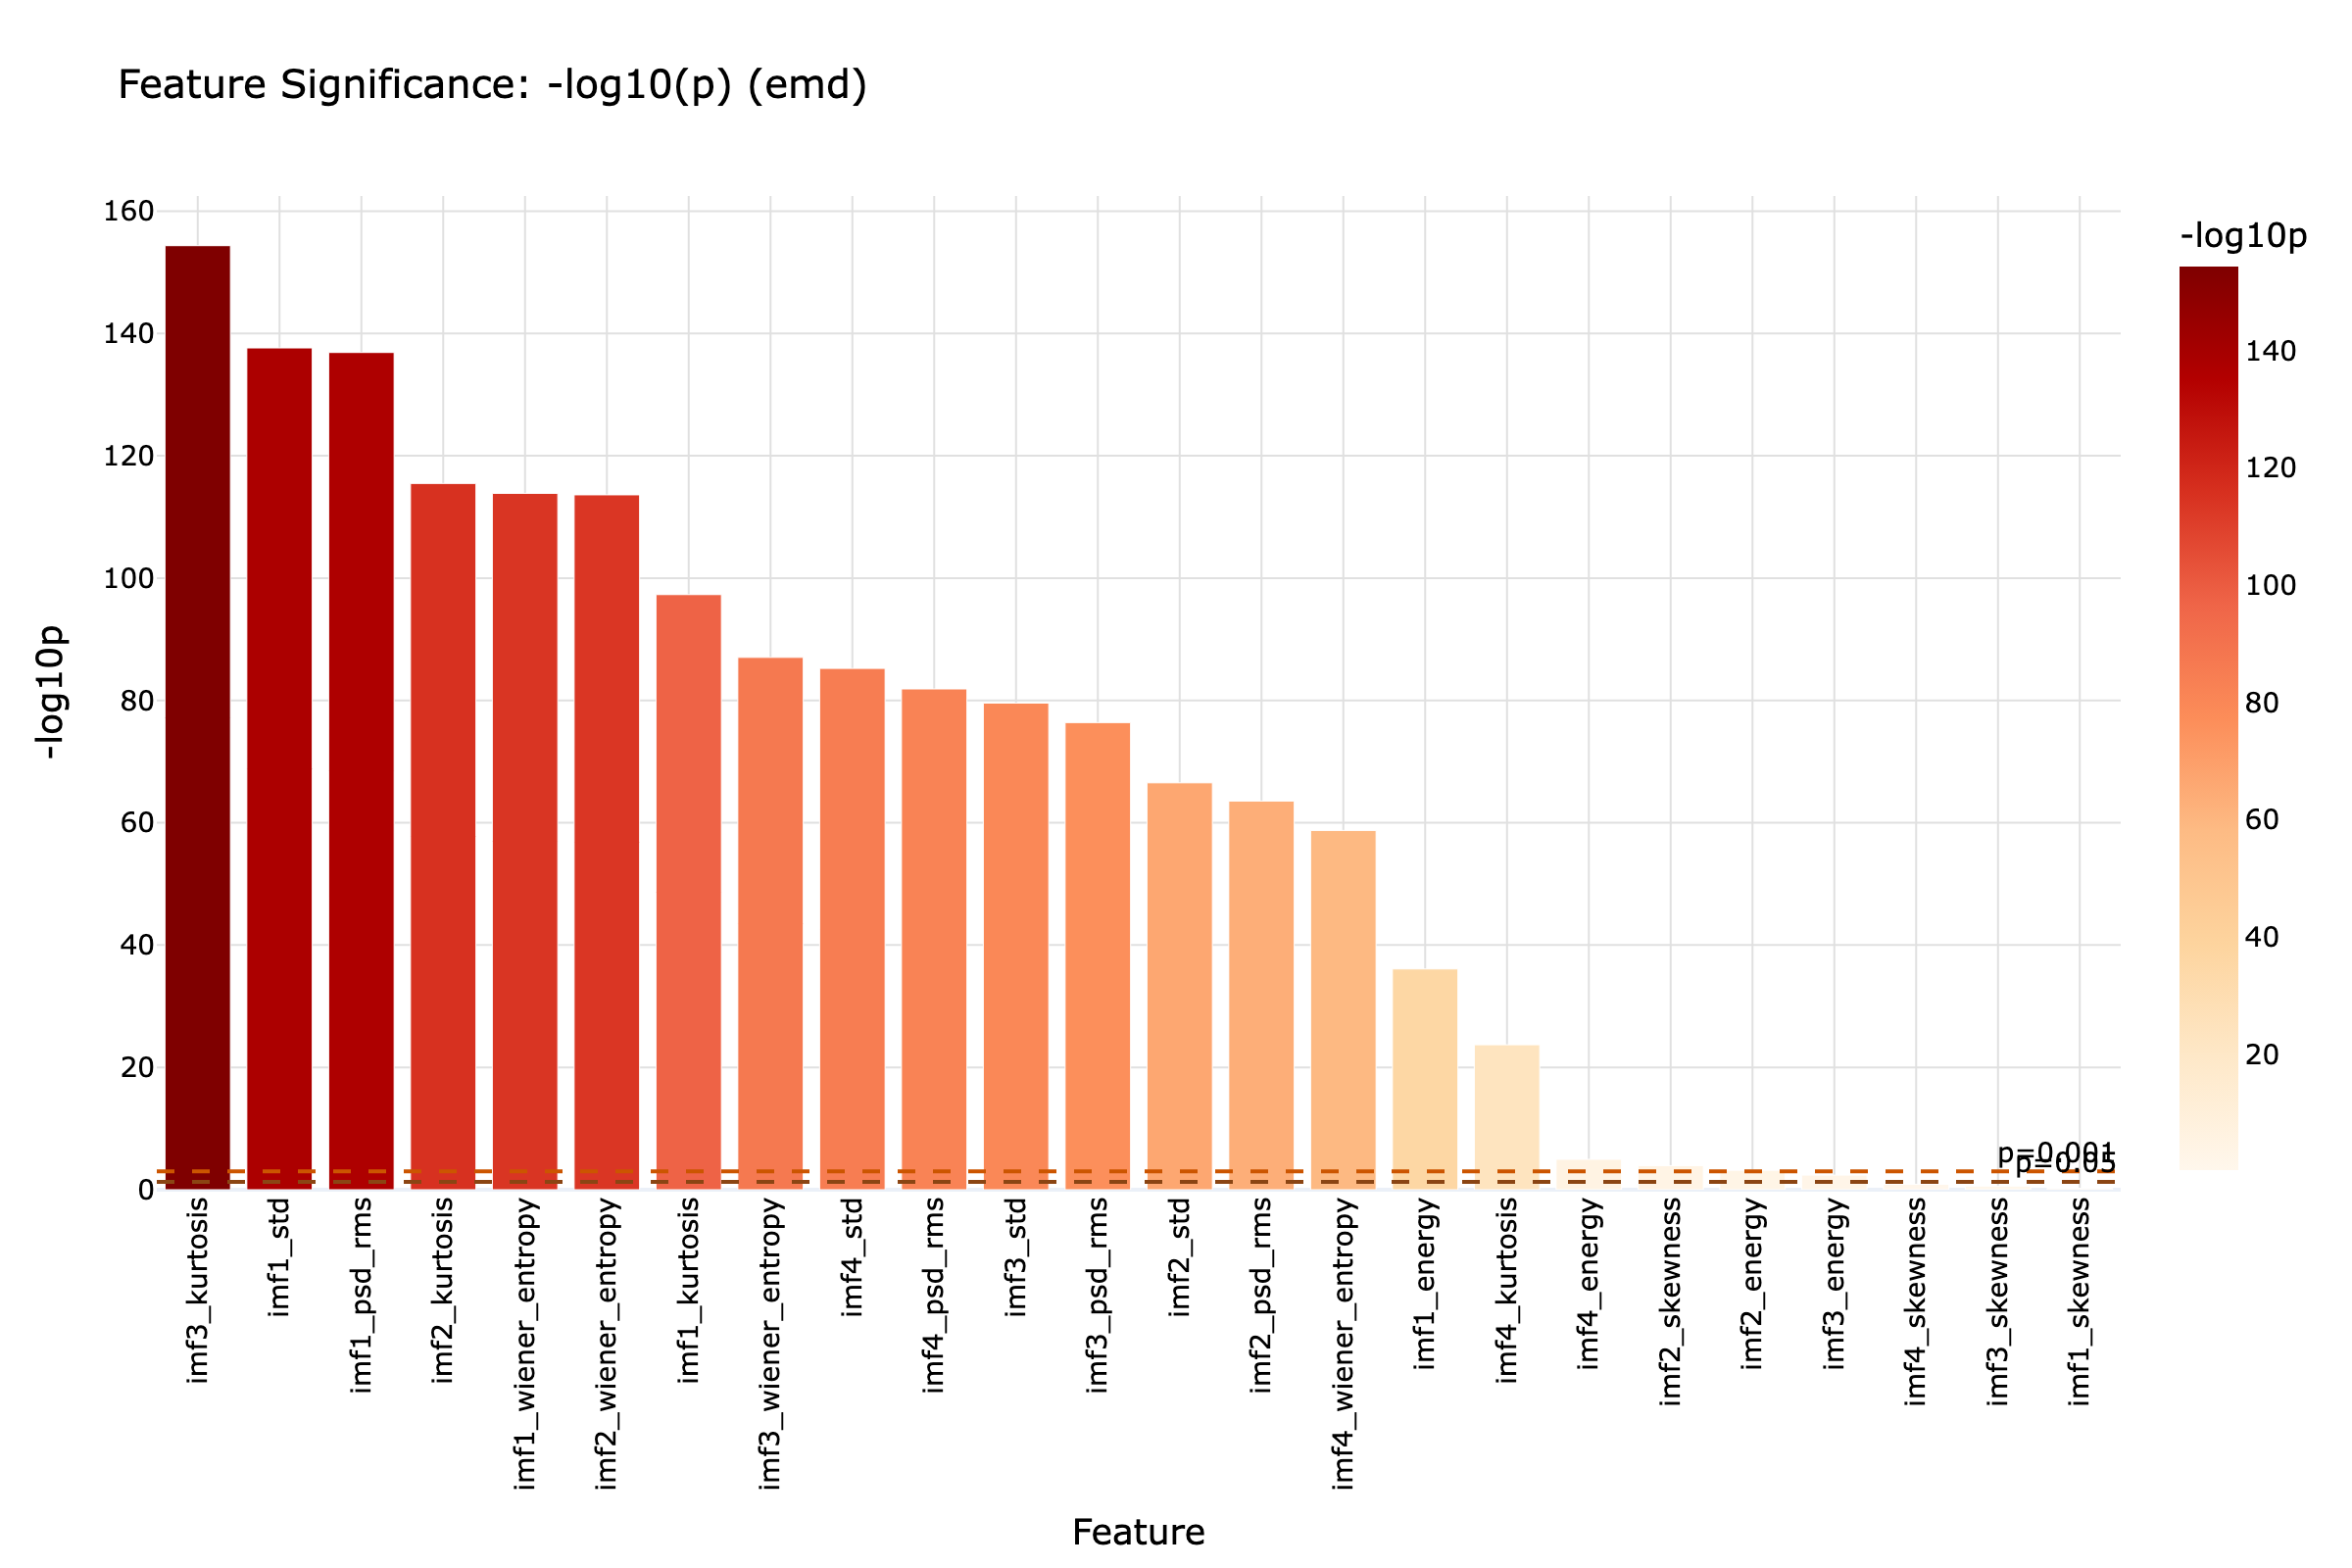
\includegraphics[width=\linewidth]{public/emd_significance.png}
        \caption{EMD features: $-\log(p)$ per principal component}
        \label{fig:emd_significance}
    \end{subfigure}
    \caption{Statistical comparison of PCA-reduced EMD features between seizure and non-seizure epochs.}
\end{figure}

Table~\ref{tab:freq_results} and Table~\ref{tab:emd_results} present the top five trials, ranked by validation accuracy, for the PCA-reduced frequency-domain and EMD feature pipelines, respectively. Each trial used a distinct random seed for data splitting to assess variability across folds.

\begin{table}[h!]
\caption{Top 5 trials -- PCA Frequency Features}\label{tab:freq_results}
{\footnotesize
\begin{tabular*}{\textwidth}{@{\extracolsep\fill}ccccccccccc}
\toprule
 & \multicolumn{5}{c}{Validation} & \multicolumn{5}{c}{Test} \\
\cmidrule(lr){2-6} \cmidrule(lr){7-11}
Trial & Acc & F1 & Prec & Rec & AUC & Acc & F1 & Prec & Rec & AUC \\
\midrule
0 & 0.762 & 0.688 & 0.683 & 0.694 & 0.807 & 0.738 & 0.731 & 0.683 & 0.786 & 0.858 \\
2 & 0.721 & 0.322 & 0.843 & 0.199 & 0.698 & 0.711 & 0.480 & 0.835 & 0.337 & 0.699 \\
8 & 0.685 & 0.554 & 0.891 & 0.402 & 0.767 & 0.718 & 0.300 & 0.864 & 0.182 & 0.808 \\
5 & 0.663 & 0.687 & 0.599 & 0.805 & 0.728 & 0.411 & 0.457 & 0.696 & 0.340 & 0.464 \\
1 & 0.639 & 0.438 & 0.614 & 0.340 & 0.658 & 0.603 & 0.503 & 0.931 & 0.345 & 0.820 \\
\botrule
\end{tabular*}
}
\end{table}

The frequency-domain pipeline achieved its highest validation accuracy of 0.762 in Trial~0, which also yielded the strongest test-set performance (accuracy 0.738, AUC 0.858, F1 0.731). Across the top five trials, test AUC ranged from 0.464 to 0.858, indicating moderate variability depending on the data split but generally favourable discriminative capacity. Precision was consistently high in several trials (e.g.\ 0.864 in Trial~8, 0.931 in Trial~1), although this sometimes came at the expense of recall, reflecting a tendency toward conservative seizure predictions.

\begin{table}[h!]
\caption{Top 5 trials -- PCA EMD Features}\label{tab:emd_results}
{\footnotesize
\begin{tabular*}{\textwidth}{@{\extracolsep\fill}ccccccccccc}
\toprule
 & \multicolumn{5}{c}{Validation} & \multicolumn{5}{c}{Test} \\
\cmidrule(lr){2-6} \cmidrule(lr){7-11}
Trial & Acc & F1 & Prec & Rec & AUC & Acc & F1 & Prec & Rec & AUC \\
\midrule
0 & 0.672 & 0.647 & 0.546 & 0.792 & 0.790 & 0.678 & 0.703 & 0.603 & 0.843 & 0.779 \\
5 & 0.655 & 0.656 & 0.605 & 0.717 & 0.712 & 0.388 & 0.392 & 0.711 & 0.270 & 0.508 \\
3 & 0.652 & 0.741 & 0.650 & 0.861 & 0.660 & 0.590 & 0.541 & 0.432 & 0.724 & 0.673 \\
8 & 0.646 & 0.638 & 0.636 & 0.639 & 0.674 & 0.602 & 0.497 & 0.430 & 0.588 & 0.643 \\
4 & 0.632 & 0.583 & 0.668 & 0.517 & 0.698 & 0.604 & 0.652 & 0.576 & 0.753 & 0.685 \\
\botrule
\end{tabular*}
}
\end{table}

The EMD pipeline exhibited lower overall accuracy than the frequency-domain approach, with a best validation accuracy of 0.672 and a corresponding test AUC of 0.779 (Trial~0). Notably, the EMD features tended to produce higher recall (e.g.\ 0.843 in Trial~0), suggesting a greater sensitivity to seizure events, albeit at the cost of reduced precision. Cross-trial variability was more pronounced, with test AUC values spanning 0.508 to 0.779.

To further visualise the performance landscape, Figures~\ref{fig:radar_plots} presents radar charts comparing the validation metrics (Accuracy, F1, Precision, Recall, AUC) for the top performing trials of both pipelines.

\begin{figure}[h!]
    \centering
    \begin{subfigure}{0.48\textwidth}
        \centering
        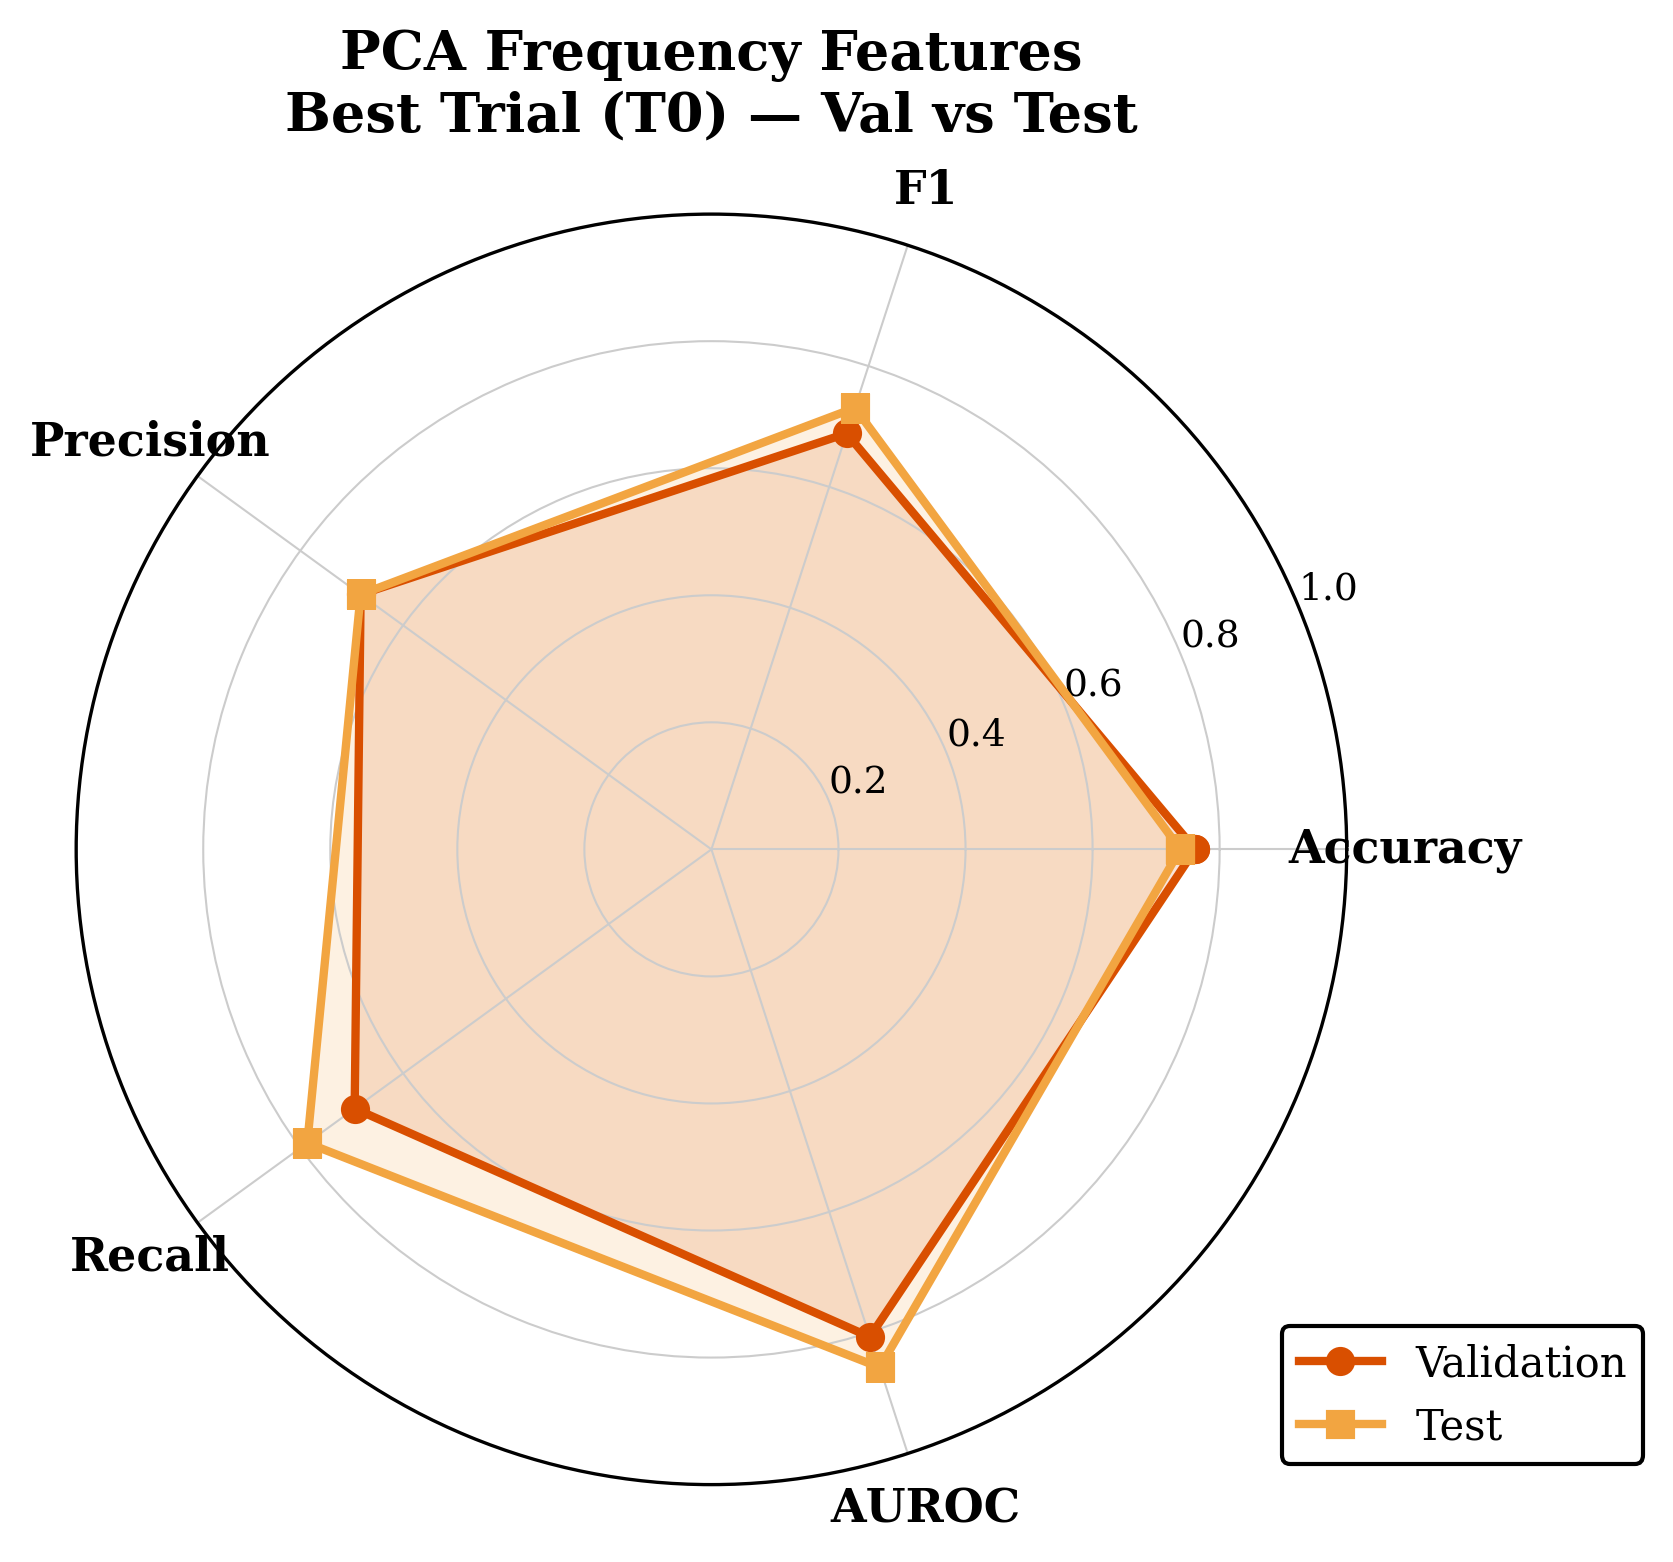
\includegraphics[width=\linewidth]{public/radar_pca_freq.png}
        \caption{Frequency Features}
        \label{fig:radar_freq}
    \end{subfigure}
    \hfill
    \begin{subfigure}{0.48\textwidth}
        \centering
        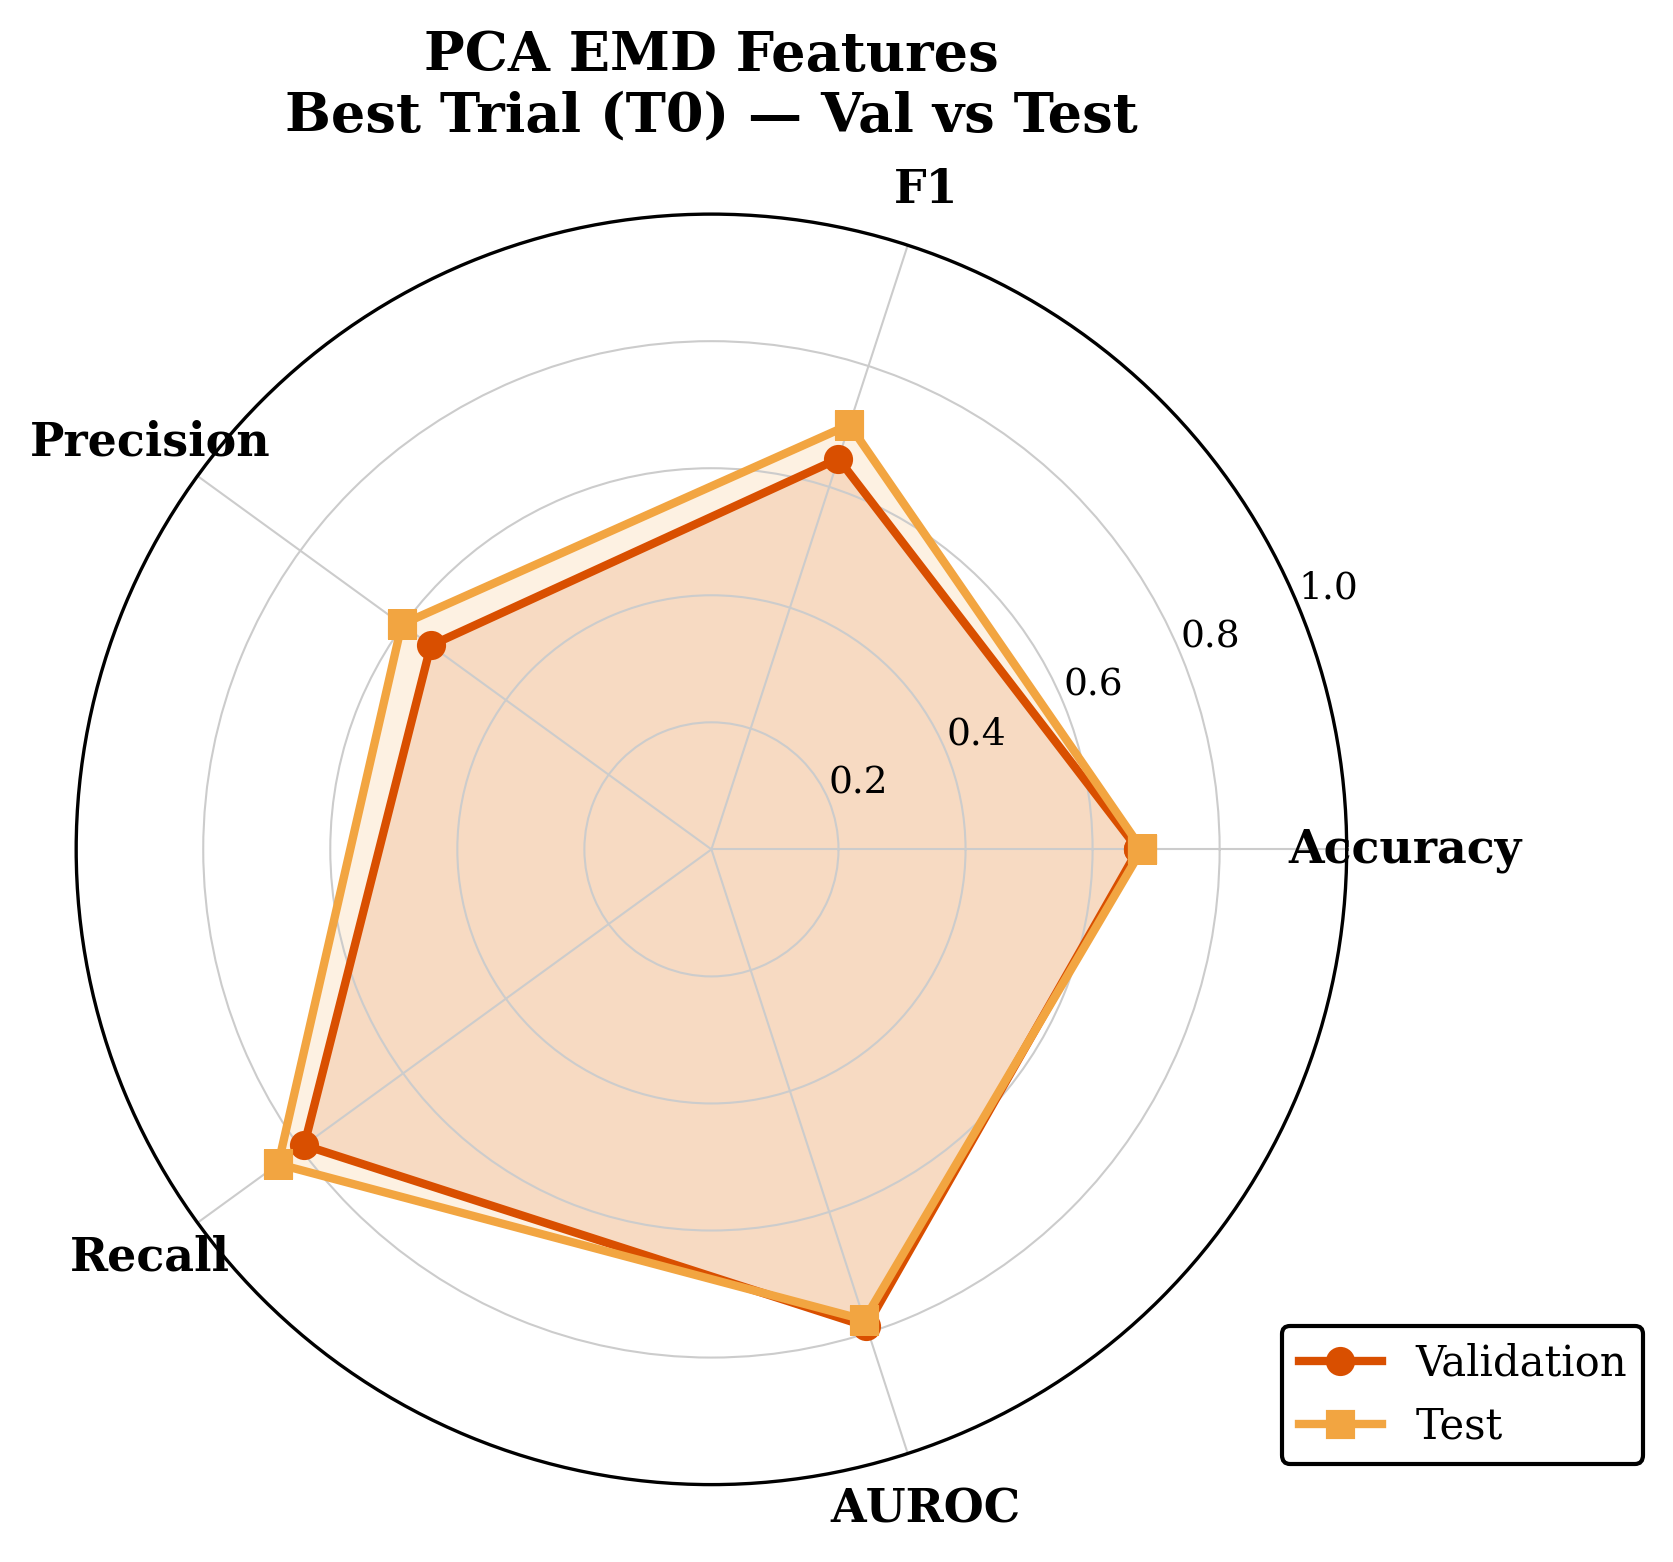
\includegraphics[width=\linewidth]{public/radar_pca_emd.png}
        \caption{EMD Features}
        \label{fig:radar_emd}
    \end{subfigure}
    \caption{Radar charts illustrating the performance profile of the top trials. The frequency-domain pipeline (a) demonstrates a more balanced profile with consistently high Area Under the Curve (AUC) and Accuracy. In contrast, the EMD pipeline (b) exhibits a distinct skew towards Recall, indicating unmatched sensitivity to seizure events despite lower overall precision.}
    \label{fig:radar_plots}
\end{figure}

The radar plots correspond with the tabular data, confirming that while the frequency-domain features provide a robust all-around classifier (larger overall polygon area), the EMD features capture complementary information that prioritises sensitivity. This structural difference in performance suggests that EMD-derived metrics may be particularly valuable in clinical screening contexts where missing a seizure (false negative) is more detrimental than a false alarm.


Discussions should be brief and focused. In some disciplines use of Discussion or `Conclusion' is interchangeable. It is not mandatory to use both. Some journals prefer a section `Results and Discussion' followed by a section `Conclusion'. Please refer to Journal-level guidance for any specific requirements. 

\section{Conclusion}\label{sec13}

Conclusions may be used to restate your hypothesis or research question, restate your major findings, explain the relevance and the added value of your work, highlight any limitations of your study, describe future directions for research and recommendations. 

In some disciplines use of Discussion or 'Conclusion' is interchangeable. It is not mandatory to use both. Please refer to Journal-level guidance for any specific requirements. 

\backmatter

\bmhead{Supplementary information}

Not applicable.

\bmhead{Acknowledgements}

Not applicable.

\section*{Declarations}

\begin{itemize}
\item \textbf{Funding:} Not applicable.
\item \textbf{Conflict of interest:} The authors declare no competing interests.
\item \textbf{Ethics approval:} Not applicable. This study used a publicly available, de-identified dataset.
\item \textbf{Data availability:} The neonatal EEG dataset used in this study is publicly available from the Zenodo repository associated with Stevenson et al.\ (2019).
\item \textbf{Code availability:} Not applicable.
\item \textbf{Author contribution:} Not applicable.
\end{itemize}

%%===========================================================================================%%
%% If you are submitting to one of the Nature Portfolio journals, using the eJP submission   %%
%% system, please include the references within the manuscript file itself. You may do this  %%
%% by copying the reference list from your .bbl file, paste it into the main manuscript .tex %%
%% file, and delete the associated \verb+\bibliography+ commands.                            %%
%%===========================================================================================%%

\bibliography{sn-bibliography}% common bib file
%% if required, the content of .bbl file can be included here once bbl is generated
% \input sn-bibliography.bib



\end{document}
